\documentclass[pre,aps,floatfix,10pt,superscriptaddress, notitlepage,preprint]{revtex4-1}
\pdfoutput=1
\usepackage[english]{babel}
\usepackage[T1]{fontenc}
\usepackage[latin9]{inputenc}
\usepackage{amsmath,amssymb}
\usepackage[svgnames]{xcolor}
\usepackage{graphicx}
\usepackage{acro}
\usepackage{subfig}
\usepackage{caption}
\graphicspath{{figures/}}

\captionsetup[figure]{justification=raggedright}

\newcommand{\set}[1]{\ensuremath{\mathcal{#1}}}

\DeclareAcronym{pdf}{
	short=PDF,
	long=Probability Density Function,
}
\DeclareAcronym{iid}{
	short=i.i.d.,
	long=Independent Identically Distributed
}
\DeclareAcronym{ou}{
	short=OU,
	long=Ornstein-Uhlenbeck,
}
\DeclareAcronym{gktl}{
	short=GKTL,
	long=Giardina-Kurchan-Tailleur-Lecomte,
}
\DeclareAcronym{ams}{
	short=AMS,
	long=Adaptive Multilevel Splitting,
}
\DeclareAcronym{tams}{
	short=TAMS,
	long=Trajectory Adaptive Multilevel Splitting,
}
\DeclareAcronym{scgf}{
	short=SCGF,
	long=Scaled Cumulant Generating Function,
}
\DeclareAcronym{lbm}{
	short=LBM,
	long=Lattice Boltzmann Method,
}
\DeclareAcronym{lbe}{
	short=LBE,
	long=Lattice Boltzmann Equation,
}
\DeclareAcronym{lgca}{
	short=LGCA,
	long=Lattice Gas Cellular Automata,
}
\DeclareAcronym{lbgk}{
	short=LBGK,
	long=Lattice Bhatnagar-Gross-Krook
}
\DeclareAcronym{OU}{
	short=O-U,
	long=Ornstein--Ulhenbeck
}
\DeclareAcronym{dns}{
	short=DNS,
	long=Direct Numerical Simulation,
}
\DeclareAcronym{md}{
	short=MD,
	long=Molecular Dynamics,
}
\DeclareAcronym{cfd}{
	short=CFD,
	long=Computational Fluid Dynamics,
}

\definecolor{myred}{HTML}{b30000}
\definecolor{mygreen}{HTML}{008000}
\newcommand{\EL}[1]{{\color{myred}{#1}}}
\newcommand{\TL}[1]{{\color{mygreen}{#1}}}

\begin{document}
	
\title{Rare-event sampling applied to the simulation of extreme mechanical efforts exerted by a turbulent flow on a bluff body}

\author{Thibault Lestang}
\email{thibault.lestang@ens-lyon.fr}
\affiliation{Univ Lyon, ENS de Lyon, Univ Claude Bernard de Lyon, CNRS, Laboratoire de Physique, F-69342 Lyon, France}
\affiliation{Univ Lyon, Ecole Centrale de Lyon, Univ Claude Bernard de Lyon, INSA de Lyon, CNRS, Laboratoire de M\'ecanique des Fluides et d'Acoustique, F-69134 Ecully cedex, France}
\author{Freddy Bouchet}
\email{freddy.bouchet@ens-lyon.fr}
\affiliation{Univ Lyon, ENS de Lyon, Univ Claude Bernard de Lyon, CNRS, Laboratoire de Physique, F-69342 Lyon, France}
\author{Emmanuel L�v�que}
\email{emmanuel.leveque@ec-lyon.fr}
\affiliation{Univ Lyon, Ecole Centrale de Lyon, Univ Claude Bernard de Lyon, INSA de Lyon, CNRS, Laboratoire de M\'ecanique des Fluides et d'Acoustique, F-69134 Ecully cedex, France}
	
	
	
\begin{abstract}
This study evaluates the relevance of rare-event sampling techniques to accelerate the simulation of extreme mechanical efforts exerted by a turbulent flow impinging onto a bluff body.
The main idea is to replace a long simulation by a set of much shorter ones, running in parallel, with dynamics that are replicated or pruned in order to sample large-amplitude events more frequently. 
%
Such techniques have been shown to be efficient for a wide range of problems in statistical physics, computer science, biochemistry, enabling the simulation of rare  events out of reach by direct sampling.
This work is the first application to fluid-structure interaction problems. 
%
The drag experienced by a squared obstacle placed in a turbulent flow (in two dimensions) is taken as a representative case study to investigate the performance of two major rare-event sampling algorithms, namely the \ac{ams} and the \ac{gktl} algorithms.
Practical evidence is given that the fast sweeping-time of fluid structures past the obstacle has a drastic influence on the efficiency of these two algorithms.
While it is shown that the \ac{ams} algorithm does not yield significant run-time savings, the \ac{gktl} algorithm appears to be efficient to sample extreme fluctuations of the time-averaged drag and estimate related statistics such as return times.
\end{abstract}
	
\maketitle
	
\section{Introduction}
	
% general comments on physical problem %
%
Turbulent flows are important in a variety of natural phenomena, industrial and civil applications with the characteristic feature to spontaneously develop intense and sporadic motions associated with extreme internal forces \cite{lesieur_book,donzis_sreenivasan_2010,Yeung}.
``Extreme'' refers here to fluctuations that can deviate from the mean value by ${\cal{O}}(10)$ standard deviations.
In engineering, the nature of such extreme dynamical events and their statistics are of crucial interest to predict excessive mechanical efforts.
Such anomalous constraints can threaten the structural integrity of embedded structures.
%

From the viewpoint of chaotic dynamical systems, turbulence in fluids is linked to non-linearity and strong departure from statistical equilibrium \cite{KRAICHNAN}.
The use of perturbative methods in identifying resonant interactions among degrees of freedom responsible for extreme fluctuations is not successful.
Simulation offers a practical approach to gain physical insight into these events, quantify their intensity and estimate their frequency of occurrence.
However, this requires very long simulations since these events are also very rare.
% general def on rare-event sampling %
%
{Rare-event sampling refer to a large body of methods that aim at sampling preferentially regions of phase space that correspond to rare events, that would otherwise be accessed with a very low probability through a brute-force sampling.}
%
Our motivation is to conduct the first computational study of extreme mechanical efforts acting on a immersed body, using both very long timeseries and rare event sampling techniques.
%	
	
% next two paragraphs may be too technical -- Find a way to summarize them in a few sentences accessible to a broad audience in fluid mechanics? Notion of action will be vague for many readers
%
In fluid turbulence, rare-event sampling has been approached mainly from simplified dynamics such as the one-dimensional Burgers' equation with a stochastic forcing \cite{bec_burgers_2007}. In that case, dynamics can be sampled by using a Markov chain Monte-Carlo algorithm \cite{duben_monte_2008,mesterhazy2011anomalous,mesterhazy2013lattice} that provides a framework for rare-event sampling.
%
An alternative approach is based on \emph{instantons} \cite{gurarie_instantons_1996,grafke2015instanton} and applies to stochastically driven systems in the limit of weak noise.
Instantons refer to the most probable trajectories (in phase space) that achieve a given rare event, in the limit of weak noise. Suitable numerical schemes can be used to evaluate instantons as well as the related probabilities of rare events \cite{chernykh_large_2001,grafke_instanton_2013,grigorio_instantons_2017,laurie2015computation,bouchet2014langevin}.
An example is the investigation of the physics of rogue waves~\cite{dematteis2018rogue,dematteis2019experimental}.
%
A drawback of the aforementioned approaches is their limitation to simple and stochastically driven dynamics.
%

%
In this paper, a more general approach is considered for complex, potentially deterministic dynamical systems.
It is based on sampling algorithms relying on \emph{selection rules} applied to an ensemble of trajectories, and designed to sample rare events of some observable with a higher frequency.
%    
%
Even though such ideas date back to the early 1950's, they have received ever-growing interest during the last 20 years with successful applications in various domains such as chemistry \cite{van_erp_elaborating_2005,escobedo_transition_2009,teo_adaptive_2016}, biophysics \cite{huber_weighted-ensemble_1996,zuckerman2017weighted,bolhuis2005kinetic}, nuclear physics \cite{louvin2017}, nonlinear dynamical systems \cite{tailleur_probing_2007} or communication networks simulation \cite{villen-altamirano_restart:_1994}.
More importantly, these type of algorithms have been shown to be useful for the study of rare events in simple deterministic dynamics~\cite{wouters2016rare}.
%

%
An original contribution of the present study is certainly the application of rare-event sampling algorithms in the context of far-from-equilibrium dynamics with an irreducible very large number of degrees of freedom. 
%Let us remark that most of previous successful applications involve dynamical systems with low-dimensional attractors. \EL{is it TRUE? \#11}
% 
Two different algorithms suitable for out-of-equilibrium dynamics are considered and compared. Namely, the Adaptive Multilevel Splitting algorithm and the Giardina-Kurchan-Tailleur-Lecomte algorithm.
%
	
The \acl{ams} algorithm \cite{cerou_adaptive_2007} inherits from old ideas about splitting approaches \cite{KahnHarris1951,glasserman_look_1998,glasserman_multilevel_1999} -- a detailed description will be given later.  
In recent years, it has allowed for the computation of rare events in problems involving a large number of degrees of freedom such as molecular dynamics simulations \cite{aristoff_adaptive_2015,teo_adaptive_2016}. The first use of the \ac{ams} algorithms for more complex dynamics, for instance stochastic partial differential equations was for the computation of rare trajectories in the Allen-Cahn equations \cite{rolland_computing_2016}. More recently is has been applied to rare events in stochastic models of wall-turbulence \cite{rolland_extremely_2018} and atmospheric dynamics \cite{bouchet2019rare}.

During the last decade, the main theoretical framework for the study of rare events in statistical physics has been the theory of large deviations \cite{touchette_large_2009}.
Alongside, numerical methods have been developed to sample rare events \cite{moral_feynman-kac_2004}. 
Among them, the \ac{gktl} algorithm \cite{giardina_direct_2006} is particularly suited for (chaotic) dynamical systems \cite{giardina_simulating_2011,Laffargue_2013}.
%
{Recently, \ac{gktl} has allowed to successfully perform the numerical simulation of extreme heat waves in a simplified modelling of the atmosphere \cite{ragone_computation_2018}. 
This achievement represents a significant leap in the applicability of rare-event sampling to complex dynamical systems. Along the same line, rare-event sampling algorithms are here pushed aside traditional applications by considering fluid-structure interaction in a turbulent flow.}
%

{The first part of this paper presents a study of the extreme fluctuations of the drag force acting on a square in a two dimensional turbulent channel flow.
  This study is based on the simulation of the flow over a very long duration, made possible by the simplicity of the flow.}
%
The motivation for this study is twofold.
First, we provide a description of the statistics and dynamics related to extreme drag fluctuations.
To the author's knowledge, such a description does not exist in the literature.
Second, this study provides reference results that can be used to validate results obtained using
rare event algorithms.

% Annonce du plan
Section~\ref{sec:test_flow} introduces the flow set-up and describes the dynamics related to typical
drag fluctuations.
The statistical properties of the drag are then discussed.
In section~\ref{sec:direct_sampling} we discuss the phenomenology of extreme fluctuations of extreme
drag fluctuations, based on a direct sampling approach.
Both the instantaneous drag and time-averaged drag are considered.
We find that sampled extreme events for the instantaneous drag display similar dynamics and we highlight that the phenomenology of extremes for the time-averaged drag can be related to the statistical properties of the instantaneous drag.
This is supported by the study of extreme events for simple stochastic dynamics.
Next, section~\ref{sec:rare_events_algorithms} describes the application of both the \ac{ams} and \ac{gktl} algorithms to the numerical simulation of extreme drag fluctuations, using the same flow set-up.
In section~\ref{sec:ams} we show that the application of the \ac{ams} to such a flow is not straightforward and connect the difficulties to the phenomenology described in the previous sections.
Section~\ref{sec:gktl} presents the computation of extremes of the time-averaged drag, using the \ac{gktl} algorithm.
Its application allows an exceptional reduction of the computational cost required to simulate trajectories corresponding to extreme time-averaged drag values.
Finally, we use the \ac{gktl} algorithm to compute the return times of extreme fluctuations of the
time-averaged drag acting on the immersed obstacle.
	
\section{Description of the numerical case study}
\label{sec:test_flow}
	
\begin{figure}
\centering
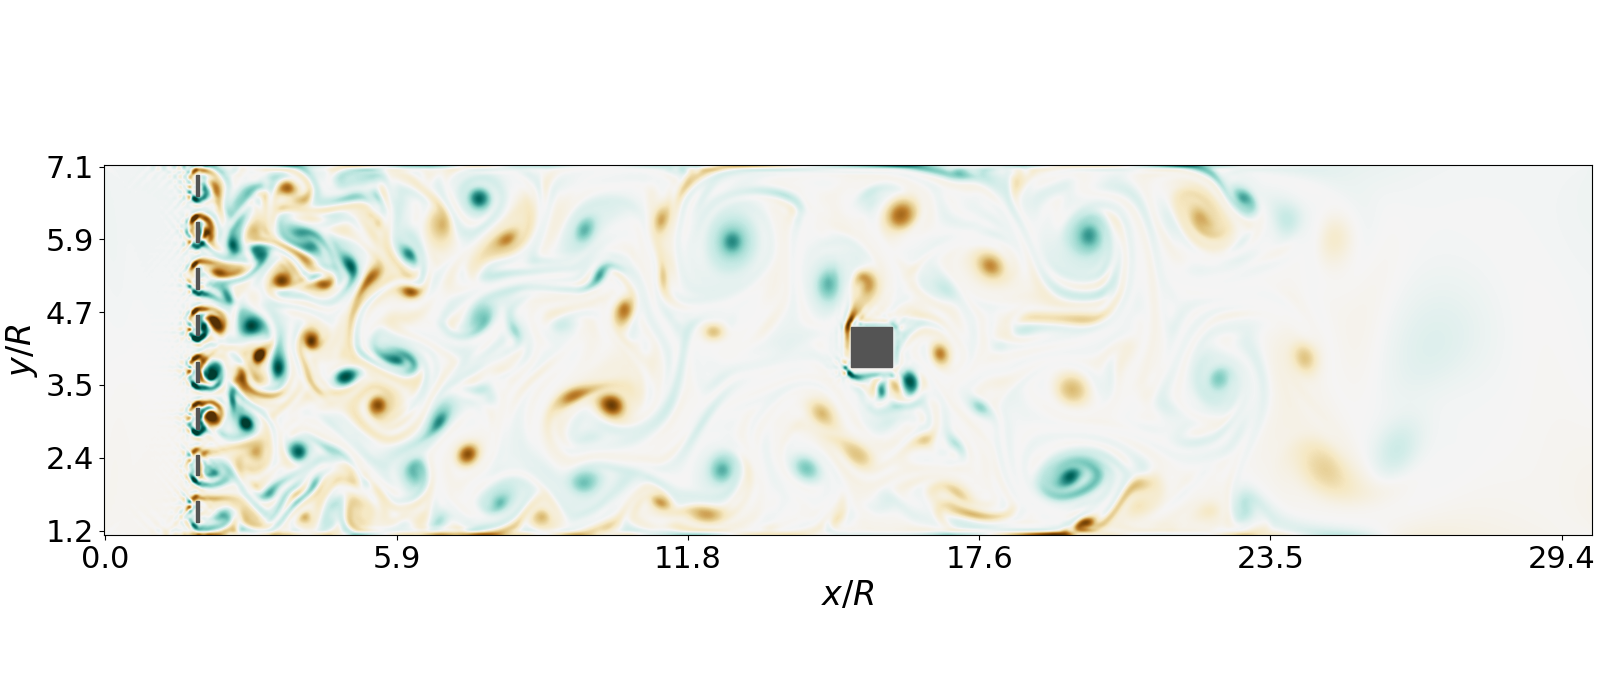
\includegraphics[width=\linewidth]{illustr_ecoulement/illustr_ecoulement}
\caption{Our case study is a grid-generated turbulent flow impinging onto a fixed squared obstacle (of size $R$) located at the centre of a channel in two dimensions. The flow is artificially damped near the end of the channel. In the developed flow, turbulent eddies have typically the size of the square, which results in strong fluctuations of mechanical efforts acting on the square. The vorticity is displayed with an arbitrary colour map from blue (negative values) to red (positive values).}
\label{fig:illustr_ecoulement}
\end{figure}
	
% introduce the flow 
%
The drag exerted by a grid-generated turbulent flow onto a fixed squared obstacle is considered as a representative case study (see Fig.~\ref{fig:illustr_ecoulement}). 
% why this flow?
%
Although real-world applications would eventually imply three-dimensional dynamics, a simplified two-dimensional setting has been chosen here to reduce the computational cost, and allow for a systematic study. 
% 
We believe that this system embeds the characteristic features that makes the application of rare-event algorithms both relevant and challenging for fluid-structure-interaction problems. 
%Namely, spatio-temporal chaos and the emergence of large-amplitude mechanical efforts on the structure.
%
% rapid description of the flow
Turbulent eddies generated in the near-wake of the grid are carried downstream.
They interact with each other and grow in size as expected for two-dimensional turbulent dynamics. 
The dimension of the grid is such that the size of the eddies that hit the square is comparable to its size, resulting in strong fluctuations of the drag acting on the square. 
%
%Finally, the obstacle does not deform or move either. 
%
%Through this simplified setting, our motivation is primarily to evaluate the operability of sampling techniques to capture extreme events with a significant run-time savings.  
%

% lattice Boltzmann method 
%
The flow dynamics is integrated by the lattice Boltzmann (LB) method in our numerical simulations. 
While traditional methods in \emph{computational fluid dynamics} rely on a discretization of the Navier-Stokes equations, the LB method considers the fluid at a mesoscopic level. Capturing the dynamics of collections of fluid particles distributed on a lattice is here preferred to solving non-linear PDEs. 
%This seems crazy, however, most details at the mesoscopic level play actually no role at the macroscopic level. Therefore, the LB algorithm may be viewed as a minimal kinetic scheme compliant to the fluid dynamics at the macroscopic level.
Further details are given in Appendix and references therein.
In our context, the LB method has been chosen principally for its computational manageability and efficiency. 


% geometry
%
The simulated flow develops in a long plane channel of dimension $513 \times 129$ mesh points. The squared obstacle has size $R=16$ (in mesh unit) and is located at the centre of the channel. The spacing and bar height of the entrance grid are both equal to $R/2$ (see Fig.~\ref{fig:illustr_ecoulement}). 
% boundary conditions
%
No-slip boundary conditions are enforced on top and bottom walls of the channel and on the surface of the obstacle by using an halfway bounce-back procedure \cite{lbm_book}.  
%
Upstream the grid, a constant parabolic velocity profile and a constant mass density (equal to unity) are imposed as inlet condition. 
The centerline velocity is $0.05$ in lattice units, \textit{i.e.} normalised by $\Delta x/\Delta t$ with $\Delta x$ and $\Delta t$ referring to the lattice resolution and the time-step respectively. The initial distributions are imposed at equilibrium (see Appendix). 
In the bulk, the viscosity is adjusted to generate grid turbulence with Reynolds number $\mathrm{Re_{grid}}=1200$. The reference Mach number is equal to $0.06$ in agreement with the assumption of weak compressibility of the LB method. 
Near the end of the channel, the flow is progressively damped within a \textit{sponge layer} where the viscosity is artificially enhanced. Finally, the outlet boundary condition relies on a second-order extrapolation of the velocity and mass density. The extrapolated distributions are evaluated through a regularization procedure relying on a finite difference estimation of the local stress tensor, as introduced in \cite{latt2008straight}. 

	
\subsection{The drag force}
\label{sec:drag_force}
	
\begin{figure}
	\centering
	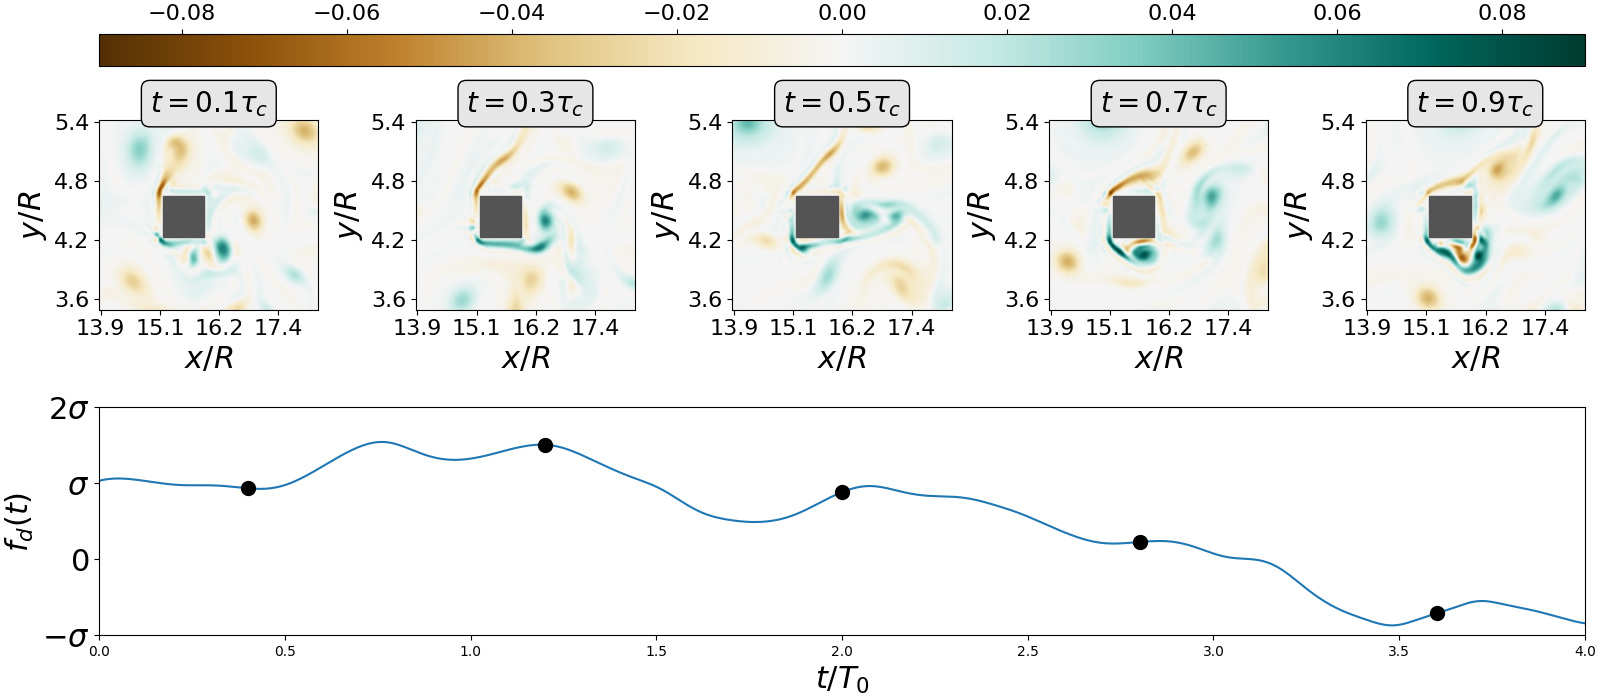
\includegraphics[width=\linewidth]{ecoulement_typique/ecoulement_typique.png}
	\caption{Snapshots of the vorticity related to typical drag fluctuations (within one standard deviation) over a time interval of length $\tau_c \simeq 4\tau_0$; $\tau_c$ will be identified later as the correlation time of the drag signal.
	The vorticity is given in lattice units.}
	\label{fig:typical_vorticity}
\end{figure}

%% LB parameters  %

% drag signal
%
The incoming turbulent flow exerts fluctuating mechanical efforts onto the squared obstacle.
The \textit{drag} is defined as the resulting force in the streamwise $x$-direction. Formally 
\begin{equation}
\label{eq:drag_definition}
f_d(t) = \int_{\mathcal{S}} \boldsymbol{\tau}_{x \beta}(\mathbf{x},t) ~ \mathrm{d}{\mathcal{S}}_\beta(\mathbf{x}),
\end{equation}
where $\mathcal{S}$ is the surface of the obstacle and $\boldsymbol{\tau}$ denotes the stress tensor (see Appendix). 
Here, the viscous stress makes a negligible contribution to the drag. The latter therefore results mostly from pressure forces.
% which are closely related to the distribution of velocity gradients in the vicinity of the obstacle (in the nearly-incompressible limit). 
%
Since the pressure on the top and bottom sides of the square applies in the normal direction, they do not contribute to the drag. 
As a consequence, the drag can eventually be expressed as the difference 
\begin{equation}
\label{eq:drag_approx}
f_d(t) = p_{fb}(t) - p_{base}(t)
\end{equation}
between the pressure integrated over the forebody, $p_{fb}(t)$, and the base of the obstacle, $p_{base}(t)$.
Pressure fluctuations are related to the dynamics of the vorticity field, as regions of strong vorticity correspond to strong local pressure gradients.
Indeed, considering a disc of constant vorticity $\omega$ with radius $a$ (Rankine vortex model), the local pressure gradient between the vortex core and a point infinitely far grows quadratically with the vorticity.

% Definition of turnover time
%
The typical timescale (turnover time) of drag fluctuations can be estimated from dimensional analysis as
\begin{equation}
\label{eq:turnover_time}
\tau_0 = \frac{R}{U},
\end{equation}
where $R$ is the size of the square and $U$ is the averaged velocity. 
%The viscosity is here discarded since viscous stress is negligible as compared to pressure forces.
%
% typical fluctuation of the drag
%
Fig.~\ref{fig:typical_vorticity} displays the typical evolution of the vorticity field around the obstacle over a few turnover times.
Because the vorticity generated along the forebody is swept away by the mean flow, the pressure field
in the vicinity of the base is only slightly perturbed.

\subsection{The drag as a random process
	%: Probability Density Function and correlation in time
}
\label{sec:pdfs}

\begin{figure}
  \centering
  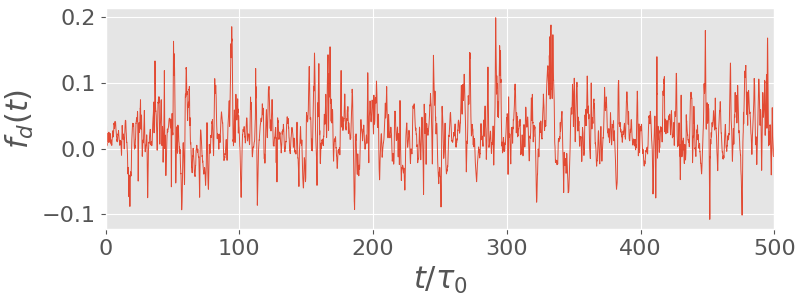
\includegraphics[width=0.7\linewidth]{typical_drag_signal/typical_drag_signal.png}
  \caption{Temporal evolution of the drag (in lattice units) acting on the square under the action of the impinging turbulent flow. The time is normalised by the turnover time related the mean-flow velocity and the size of the obstacle, \emph{i.e.} $\tau_0=R/U$.}
  \label{fig:typical_drag_signal}
\end{figure}



% drag signal
%
% Description du signal de trainee typique
Fig.~\ref{fig:typical_drag_signal} shows the time signal of the drag acting on the square, $f_d(t)$, over five hundred turnover times.
The signal appears unpredictable in details and exhibits repeated bursts of high amplitude that deviate significantly from the averaged value.
Therefore, it is  natural to model the drag as a (scalar) random process.

% drag statistics
% pdf
Drag fluctuations have been sampled along a simulation of duration $T_{tot} = 4\times 10^6~\tau_0$. This long simulation will be referred to as the \textit{control run} in the following.
It has been made possible by the relative simplicity of the investigated flow and the computational efficiency of the lattice Boltzmann method. 
The \ac{pdf} of drag fluctuations is shown in Fig.~\ref{fig:pdf_drag_a}.
It deviates from a normal law and shows an exponential tail for large positive fluctuations, \textit{i.e.}  ${\mathbb{P}}(f_d) \propto e^{-\lambda f_d}$.
%
Fig.~\ref{fig:pdf_drag_a} also displays the \ac{pdf} of drag fluctuations acting on a control surface corresponding to the periphery of the obstacle but in the absence of the obstacle. 
%
In that case, the \ac{pdf} is quasi-symmetric and does not display exponential tails. This shows that the asymmetry of the \ac{pdf} and the development of a positive exponential tail are closely related to the no-slip condition on the obstacle boundary.
\begin{figure}
  \centering
    \subfloat[\ac{pdf} of (zero-mean) drag fluctuations]
    {\label{fig:pdf_drag_a}
    	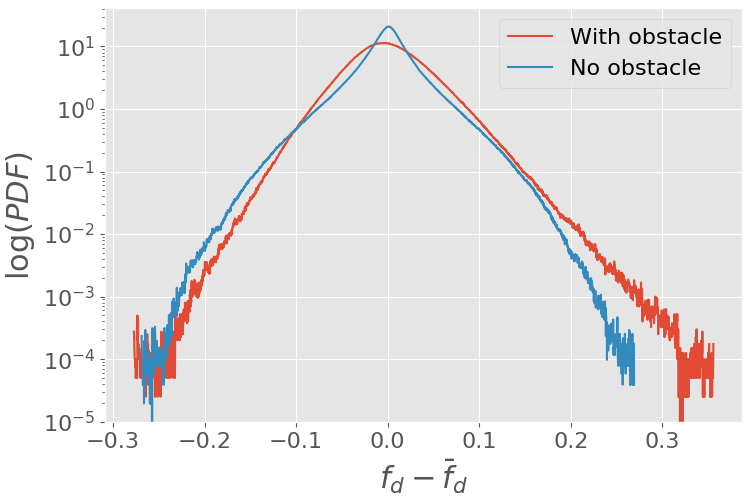
\includegraphics[width=.45\linewidth]{./PDF_drag/PDF_drag.png}}
    \subfloat[Autocorrelation of drag fluctuations]
    {\label{fig:pdf_drag_b}
    	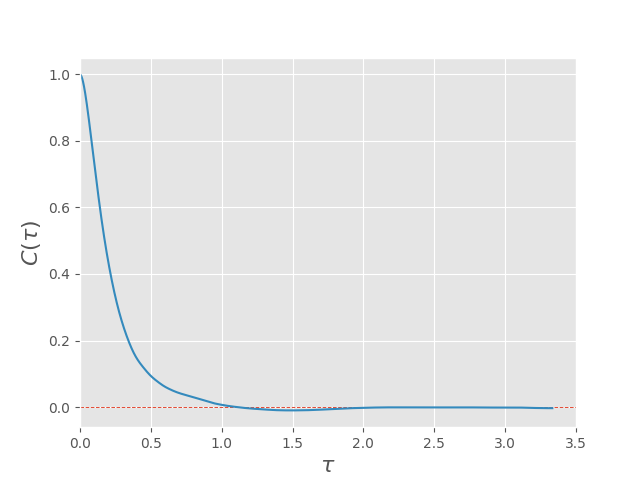
\includegraphics[width=.45\linewidth]{./autocorr_drag/autocorr_drag.png}}  
      \caption{\textbf{(a)} \ac{pdf} of (zero-mean) drag fluctuations $\tilde f_d \equiv f_d - \bar{f_d}$ where $\bar{f_d}$ denotes the time-averaged value. The drag is evaluated both in the presence (red) and in the absence (blue) of the obstacle. %Note that the amplitudes have not been normalized.
  \textbf{(b)} Autocorrelation function of the drag defined as $C(\tau) = \overline{ \tilde f_d(t+\tau)\tilde f_d(t)} ~/~ \overline{{\tilde f_d}^2}$. The correlation time $\tau_c\simeq 4 \tau_0$ is defined by the condition $C(\tau_c)=0$.
  %$\tau_c$ may therefore be considered as the correlation time of the drag signal.
}
  \label{fig:pdf_drag}
\end{figure}

% drag statistics
% correlation time
Lastly, the autocorrelation function of the drag $C(\tau)$ is shown in Fig.~\ref{fig:pdf_drag_b}. It is found that drag fluctuations are correlated over a time interval $\tau_c \simeq 4\tau_0$. One can argue that the drag looses its memory  over a time scale corresponding to the sweeping of a few eddies past the obstacle.
%
This observation is important for the application of rare-event algorithms as will be discussed in section~\ref{sec:rare_events_algorithms}.
%
In the following, $\tau_c$ will be referred to as the \textit{correlation time} of the drag. The ratio $\tau_0 / \tau_c$ may be viewed as a {Strouhal number}. The value $St=0.25$ is consistent with common observations for flows past blunt structures at comparable Reynolds numbers.

\section{Extreme fluctuations of the drag by means of direct sampling}
\label{sec:direct_sampling}

\begin{figure}
	\centering
	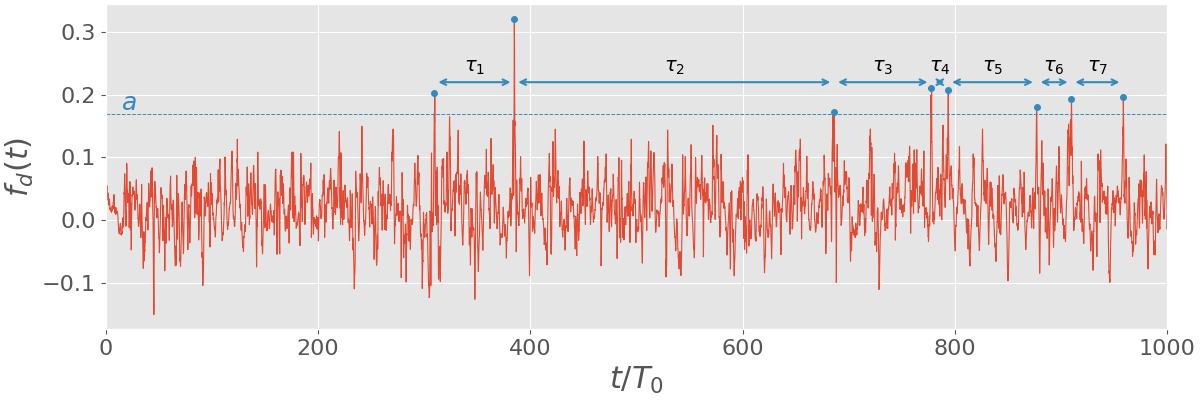
\includegraphics[width=\linewidth]{illustrate_return_time/illustrate_return_time}
	\caption{\label{fig:illustrate_return_time} {The \textit{return time} $r(a)$  is the averaged waiting time between the occurrence of peak fluctuations of amplitude larger than $a$.
	One observes that $r(a) >> \tau_c$ (correlation time) if $a$ is sufficiently large. The selected peak fluctuations are therefore well separated.}
	}
\end{figure}

\begin{figure}
	\centering
	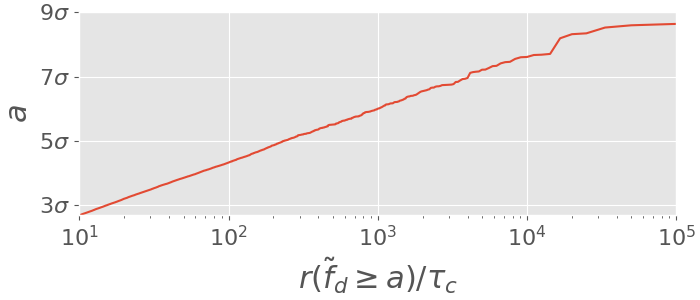
\includegraphics[width=.6\linewidth]{return_time/return_time.png}
	\caption{Amplitude of drag fluctuations as a function the corresponding return time. $\tilde{f}_d$ denotes the drag with zero mean, \textit{i.e.} $\tilde{f}_d = f_d - \overline{f_d}$.
	}
	\label{fig:return_time_instant}
\end{figure}

% return time given from direct sampling
%
The phenomenology of extreme fluctuations of the drag is first investigated through brute-force direct sampling applied to the control run.
Direct sampling is here used as opposed to approaches involving rare-events algorithms discussed in section~\ref{sec:rare_events_algorithms}.
It will provide a trustworthy baseline for the validation of rare-events algorithms. 

{\bf The waiting times $\tau$ are defined as the time between two consecutive occurrences of peak fluctuations with amplitude $f_d \geq a$, as illustrated in Fig.~\ref{fig:illustrate_return_time}.  The mixing time $\tau_m$ is the time needed for the dynamics to loose the memory of its initial conditions. As soon as the typical waiting times are much larger than the mixing time $\tau_m$, the occurrences of such events follow a Poisson process and the distribution of the waiting times is exponential: $P(\tau)=\lambda(a)\exp(-\lambda(a)\tau)$, where $r(a)=1/\lambda(a)$ is the average waiting time \cite{lestang_computing_2018}. $r(a)$ is called the {\it return time} of the level $a$. For systems without multistability, it is often the case that the mixing time $\tau_m$ is of the order of the correlation time $\tau_c$.

How rare is a fluctuation $a$ is quantified by its return time $r(a)$. We can define extreme drag fluctuations as \textit{rare events} in the sense that the return time is much larger than the correlation time, \emph{i.e.} $r(a) \gg \tau_c$.

The shape of the return time $r$ as a function of the return level $a$ is system dependent. It is often the case that  $r(a) = t(a)/\mathbb{P}(f_d\geq a)$, where the level dependent time scale $t(a)$, expected to be of order $\tau_c$, changes much more slowly with $a$ that the PDF ${\mathbb{P}(f_d\geq a)}$, for large values of $a$. As the PDF ${\mathbb{P}(f_d\geq a)}$ was shown to be well approximated by an exponential (see figure Fig.~\ref{fig:pdf_drag}), we might expect that 
\begin{equation}
 \label{eq:return_time}
r(a) \underset{a\to\infty}{\propto} \exp(-la)
\end{equation}
where $l$ is the rate describing the positive tail of the \ac{pdf} of the drag (shown in Fig.~\ref{fig:pdf_drag}).
Fig.~\ref{fig:return_time_instant} shows the evolution of the return time $r(a)$ with the amplitude of fluctuation $a$, computed from {direct sampling} of the drag signal $f_d(t)$ \cite{lestang_computing_2018}. It is consistently found that the return time $r(a)$ is well approximated by an exponential for large levels $a$. Let us also point out some deviation from the exponential law at the largest levels, that are probably the consequence of undersampling.
}
% typically for $a \gtrsim 8 \sigma$ with $\sigma$ being the standard deviation. 



\subsection{Extracting extreme drag fluctuations from a very long timeseries}
\label{sec:extreme_extraction}

% intro
%
We have extracted  the fluctuations of the drag with a return time $r(a)$ greater than  $10^4\tau_c$ from the control time-series $\{f_d(t)\}_{0 \leq t \leq T_{tot}}$. This set will be considered as representative of \emph{extreme events} in the upcoming study. The choice of this particular threshold has been driven by the need to collect enough events with large amplitude and possibly identify generic features.
%
According to Fig.~\ref{fig:return_time_instant}, the related amplitude $a$ is found equal to $7.6~\sigma$ with $\sigma$ being the standard deviation. Precisely, 104 independent fluctuations with $f_d(t) \geq 7.6\sigma$ have been identified. Each fluctuation is characterized by its maximal value, $f_d^{\star}$, and the time, $t^{\star}$, at which this maximum is reached.
%
In the following, the phenomenology of extreme drag fluctuations will be examined on the basis of this set of events.

\subsection{Instantaneous drag}
\label{sec:instantaneous_drag}

\subsubsection{Contribution of forebody and base pressure fluctuations to the overall drag fluctuation}
\label{sec:forebody_and_base_contribution}

\begin{figure}
	\centering
	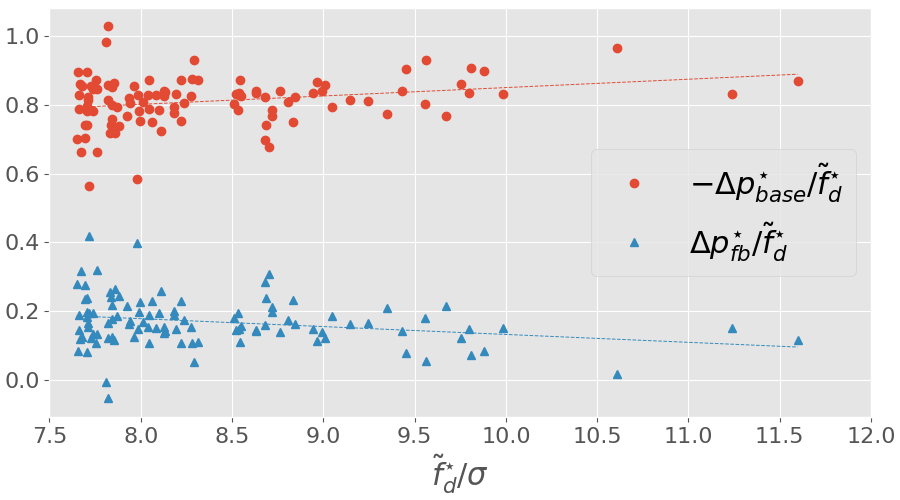
\includegraphics[width=.8\linewidth]{pressure_ratio/pressure_ratio.png}
	\caption{\label{fig:pressure_ratio} Relative contributions of the forebody and base pressure variations to extreme amplitudes of the drag. An extreme event corresponds to an amplitude $\tilde f^{\star}_d$ and a unique pair  ($\tilde{p}^{\star}_{base}$,~$\tilde{p}^{\star}_{fb}$).
	As the amplitude of the drag increases, the relative variation of the base pressure also increases. 
	%\TL{in Figure, $\tilde{p}_{fb}^{\star}/\tilde{f}_d^{\star}$ and $-\tilde{p}_{base}^{\star}/\tilde{f}_d^{\star}$} 
}
\end{figure}

% teasing
%
In section~\ref{sec:test_flow}, it was pointed out that typical drag fluctuations were originating mostly from the variation of the forebody pressure, \textit{i.e.} from the upstream turbulent flow. We shall see that the situation is different in the case of {extreme} drag fluctuations. 

% relative contribution of forebody and base pressure
%
Let $(t^{\star}, f_d^{\star})$ refer to an extreme drag event.
The (zero-mean) fluctuation $\tilde{f}_d^{\star} = f_d^{\star} - \overline{f_d}$ can be  decomposed into 
\begin{equation}
  \tilde{f}_d^{\star} = \Delta p_{fb}^{\star} - \Delta p_{base}^{\star}
\end{equation}
where $\Delta p_{fb}^{\star}$ and $\Delta p_{base}^{\star}$ denote the variations of the forebody and base pressure, respectively.
%
Fig.~\ref{fig:pressure_ratio} displays the relative contributions
$\Delta p_{fb}^{\star}/\tilde{f}_d^{\star}$ and $-\Delta p_{base}^{\star}/\tilde{f}_d^{\star}$ to the overall drag fluctuation $\tilde f_d^{\star}$.
%
It is found that the base pressure variation contributes typically to $80\%$ of the overall drag fluctuation.
Therefore, extreme amplitudes of the drag are dominated by the variation of the pressure in the vicinity of the base of the obstacle, \emph{i.e.} downstream of the obstacle.
Furthermore, Fig.~\ref{fig:pressure_ratio} suggests that the larger the fluctuation, the more important is the relative contribution of the base pressure. 
%relatively to the forebody pressure.


\subsubsection{Fluid dynamics related to extreme drag fluctuations}
\label{sec:dynamical_aspects}

\begin{figure}
	\centering
	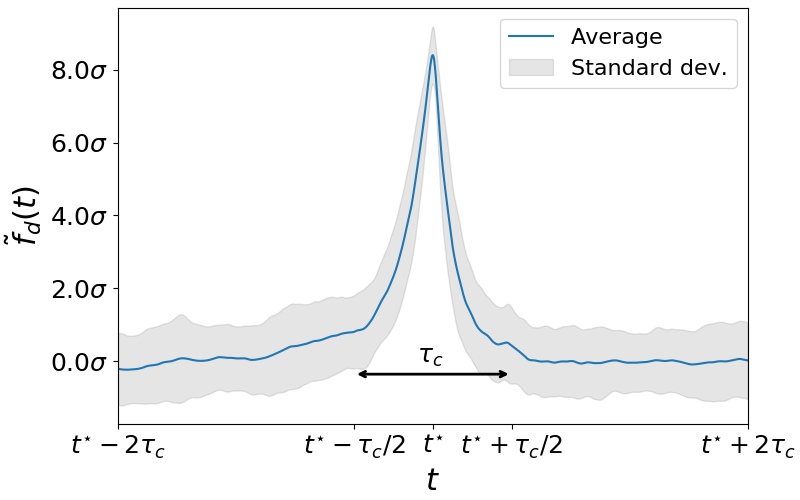
\includegraphics[width=.7\linewidth]{timeseries_extremes/timeseries_extremes.png}
	\caption{\label{fig:timeseries_extremes} Ensemble average of drag signals centred around extreme fluctuations occurring  at $t=t^{\star}$. The blue line shows the mean profile whereas the shaded area indicates variations (around the mean profile) within one standard deviation. Extreme drag events exhibit a typical lifetime of one correlation time $\tau_c$. The profile is slightly skewed indicating that the step up is slower than the return to typical values.}
\end{figure}

% mean profile around burst
%
The focus is now on the flow scenarii that yield extreme values of the drag. 
Fig.~\ref{fig:timeseries_extremes} displays the mean profile (in time) of the drag signal around extreme events. A peaked profile is observed with a width roughly corresponding to one correlation time $\tau_c$. This shows that the duration of extreme events corresponds typically to the sweeping time of the flow past the obstacle. 
%Starting from typical values, extreme drags are typically reached in less than a correlation time. 
Interestingly, the profile is also slightly skewed indicating that the step up of the drag  is slower than the return to typical values past the peak value. This is reminiscent of time-irreversibility in turbulent dynamics. 
%Moreover, such very high drag levels do not persist over time.
To better understand the flow scenarii leading to these events, the vorticity fields around the obstacle are now examined.

\begin{figure}
  \centering
  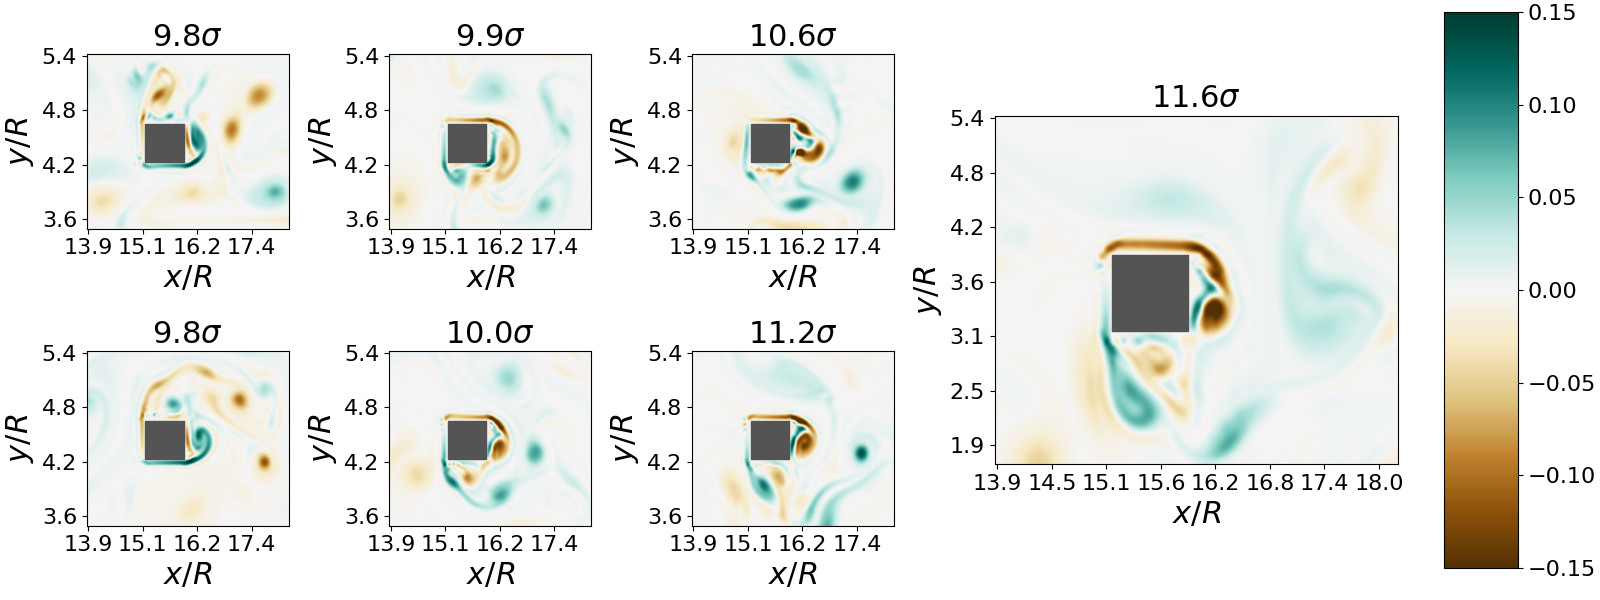
\includegraphics[width=\linewidth]{illustr_extrms_vorticity/illustr_extrms_vorticity.png}
  \caption{\label{fig:top_4_events_vorticity} Vorticity field (in lattice units) around the obstacle at $t=t^{\star}$ for the highest drag amplitudes recorded in the control run.
  }
\end{figure}

\begin{figure}
  \centering
  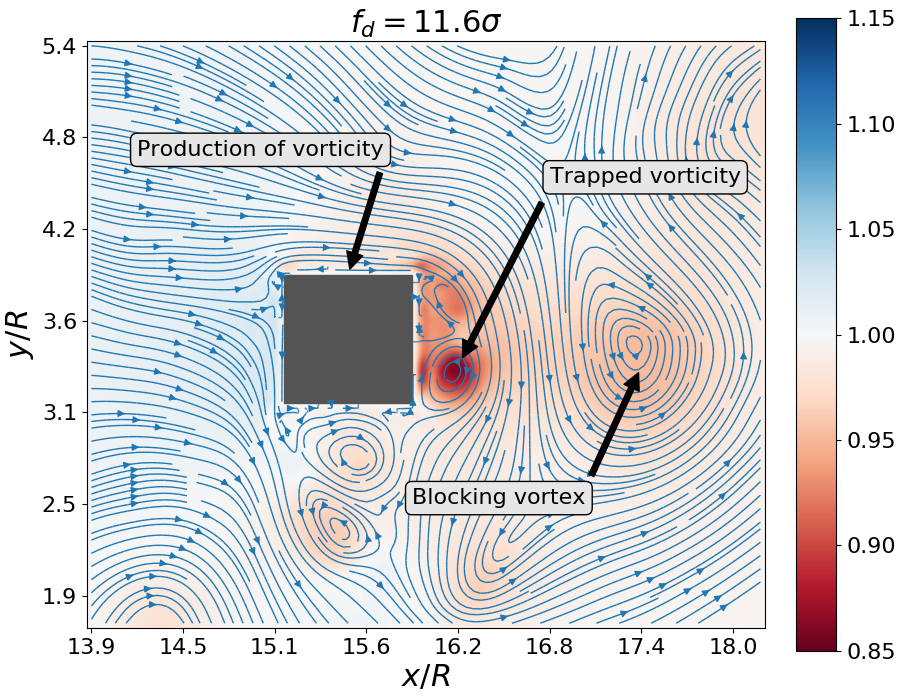
\includegraphics[width=.5\linewidth]{illustr_density_streamlines/illustr_density_streamlines.png}
  \caption{\label{fig:density+streamlines} Pressure field (in lattice units) and velocity streamlines at $t=t^{\star}$. In the near wake of the square, a (blocking) vortex blocks an intense vortex against the base of the obstacle.}
\end{figure}



\begin{figure}
  \centering
  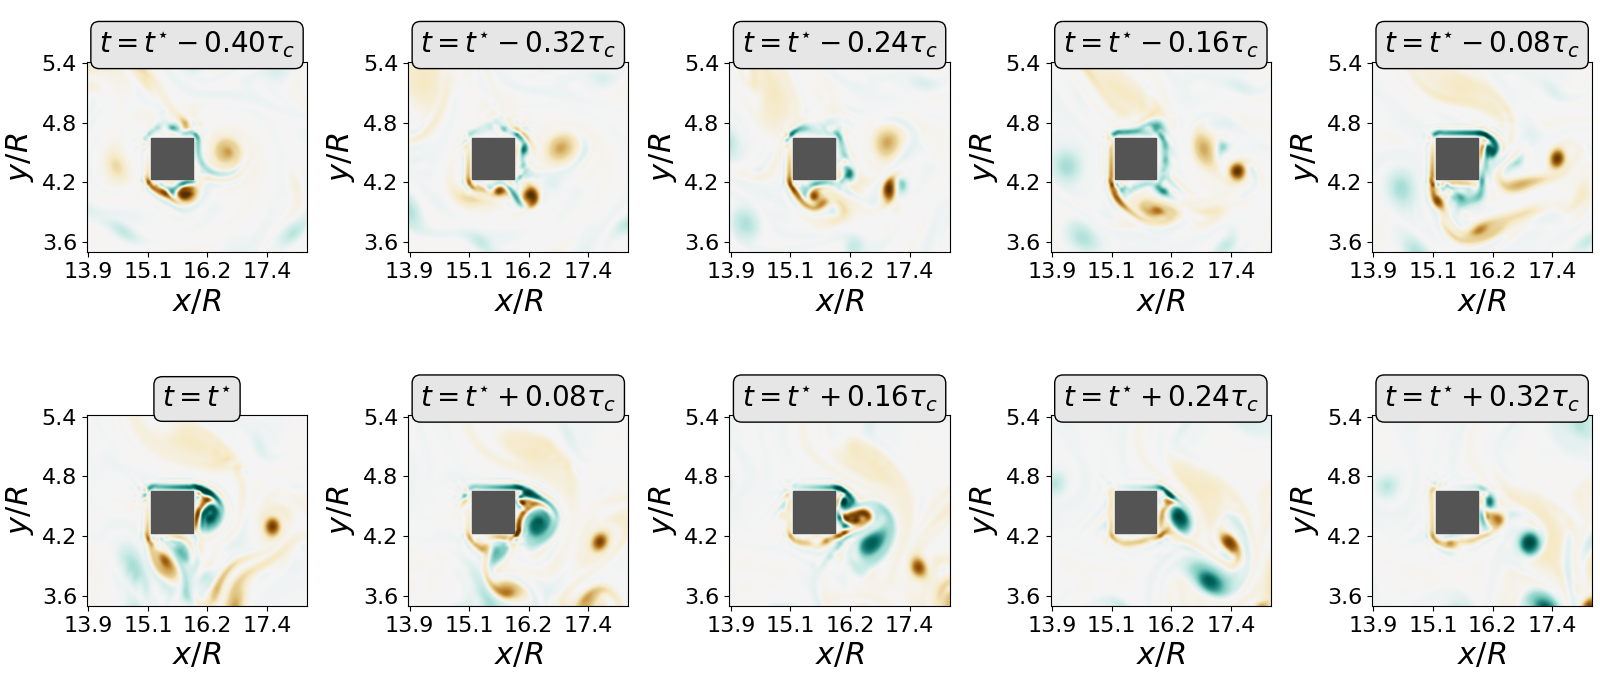
\includegraphics[width=.8\linewidth]{dynamics_extremes/dynamics_extremes.png}
  \caption{\label{fig:vorticity_dynamics} Snapshots of the vorticity field (in lattice units)  around $t=t^{\star}$.}
\end{figure}
% flow scenario
%
Fig.~\ref{fig:top_4_events_vorticity} displays the vorticity field (in lattice units) around the obstacle for the highest amplitudes of the drag during the control run.
%
In each case, an intense vortical structure is visible near the base of the obstacle.
The vorticity level of this structure is typically twice the amplitude of typical vorticity fluctuations observed in Fig.~\ref{fig:typical_vorticity}.
%
The formation of this vortex originates from an intense negative (or positive) vorticity layer at the top (or bottom) boundary of the obstacle. 
%
This high vorticity is responsible for a significant pressure drop at the base of the obstacle and, therefore, a strong drag. In contrast, nothing special happens near the forebody of the obstacle during extreme-drag events.  


The high pressure drop on the base of the obstacle appears to be closely related to the presence of a strong vortex blocked against the base. 
As illustrated in Fig.~\ref{fig:density+streamlines}, this blockage is enforced by the presence of opposite vorticity in the near wake, which holds the vortex against the base of the obstacle and prevents it from being swept away for a while.
% 
This scenario is better evidenced in Fig.~\ref{fig:vorticity_dynamics}, where the time history of the vorticity field around $t=t^\star$ for the same event is shown. 
%
Before the occurrence of the extreme event, positive vorticity originating from the bottom boundary layer develops in the near wake of the square. This positive vorticity  prevents the shedding of negative vorticity and enforces the development of a intense vortex against the base of the square. 
When the blocking vortex is in turn advected downstream, the vortex against the base is released.
%
Consistently, one can argue that the typical duration of this scenario is related to the sweeping time of the flow past the obstacle, and is therefore of the order of $\tau_c$.
This is in full agreement with the typical duration obtained from statistical consideration on the mean profile of large-drag fluctuations in Fig.~\ref{fig:timeseries_extremes}.
This scenario is generic and has been observed for most extreme events sampled in the control run.

%We found that $80\%$ of the extreme events sampled from the control timeseries can be related to very similar dynamics.

\begin{figure}
	\centering
	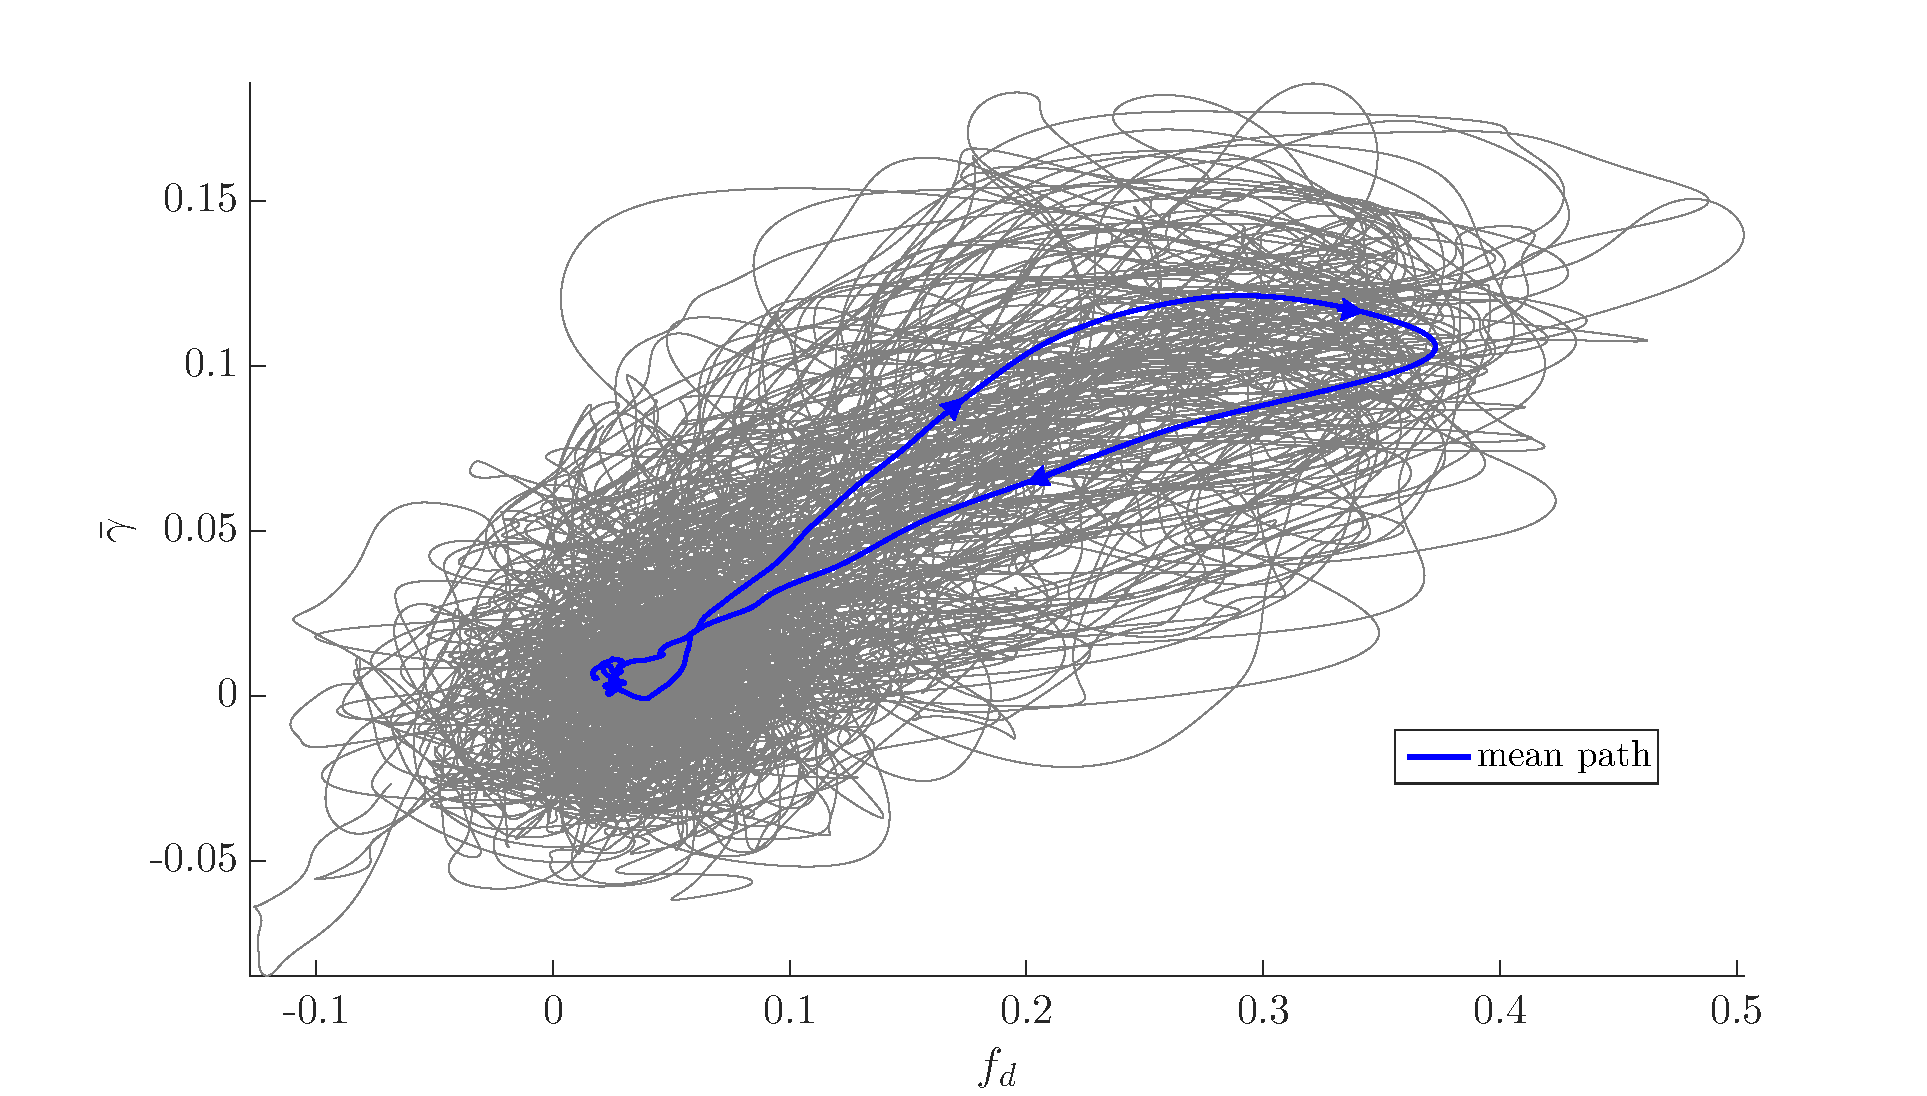
\includegraphics[width=.7\linewidth]{shear_asof_drag/shear_asof_drag}
	\caption{\label{fig:shear_asof_drag} Evolution of the (integrated) shear along the top or bottom sides of the obstacle as a function of the drag for $t^{\star}-2\tau_c \leq t \leq t^{\star}-2\tau_c$. Each trajectory corresponds to an event. The blue line is the mean path averaged over the set of extreme events sampled in the control run.}
\end{figure}


Since the occurrence of large drag amplitudes arises from the production of vorticity along the top or bottom side of the square, it is  proposed to characterize the dynamics of extreme events by their trajectory in the parameter space $(f_d(t), \bar{\gamma}(t))$ where $\bar{\gamma}(t)$ is the averaged shear along the top or bottom boundary of the square,
\begin{equation}
  \label{eq:avg_shear_def}
  \overline{\gamma} = \frac{1}{R} \int_{\mathcal{S}_\parallel} \frac{\partial u(\mathbf{x})}{\partial y}\mathrm{d}\mathbf{x},
\end{equation}
where $R$ denotes the size of the square, $u$ is the streamwise component of the velocity field and $\mathcal{S}_\parallel$ is the surface of either the top or the bottom boundary.
%
% Figure~\ref{fig:type_1_and_type_2_a} displays the label of the 104 sampled events, sorted according to the amplitude of the corresponding fluctuation.
% It illustrates that the dynamics corresponding to the large majority of events also corresponds to the events with the highest fluctuation amplitude.
%
Fig.~\ref{fig:shear_asof_drag} shows $\overline{\gamma}(t)$ as a function of the instantaneous drag $f_d$(t) for $t^{\star}-2\tau_c \leq t \leq  t^{\star}+2\tau_c$ for the 104 sampled extreme events.
Before and after the extremal fluctuation, \textit{i.e.} for $t^{\star}-2\tau_c \leq t \leq t^{\star}-\tau_c$ and $t^{\star}+\tau_c \leq t \leq t^{\star}+2\tau_c$, paths wander in a region related to typical values of both $\overline{\gamma}$ and $f_d$.
On the contrary, the drag abruptly varies for $t^{\star}-\tau_c \leq t \leq t^{\star}+\tau_c$ near the extremal amplitude.
%Paths in the $(f_d, \bar{\gamma})$ space display excursions to atypical values for both $\bar{\gamma}$ and $f_d$.
These excursions always go clockwise, that is, $\overline{\gamma}$ attains its maximum value before $f_d$ does. 
This is consistent with an increase of $\overline{\gamma}$ acting as a precursor for extreme drag fluctuations.
In this representation, we also observe that the path related to the increase of the drag is longer than the path related to the return to typical values. 


%The remaining $20\%$ of the sampled events correspond to slightly different dynamics. In this case the vorticity responsible for the base pressure drop is not created along the top or bottom boundary, but directly through viscous shear alongside the base boundary of the obstacle. This viscous shear is induced by a large vortex detached from the obstacle. For a more detailed description of such dynamics, see chapter 3 of~\cite{lestang:tel-01974316}.








\subsection{Extreme fluctuations of the time-averaged drag }
\label{sec:time_avg}


\begin{figure}
	\centering
	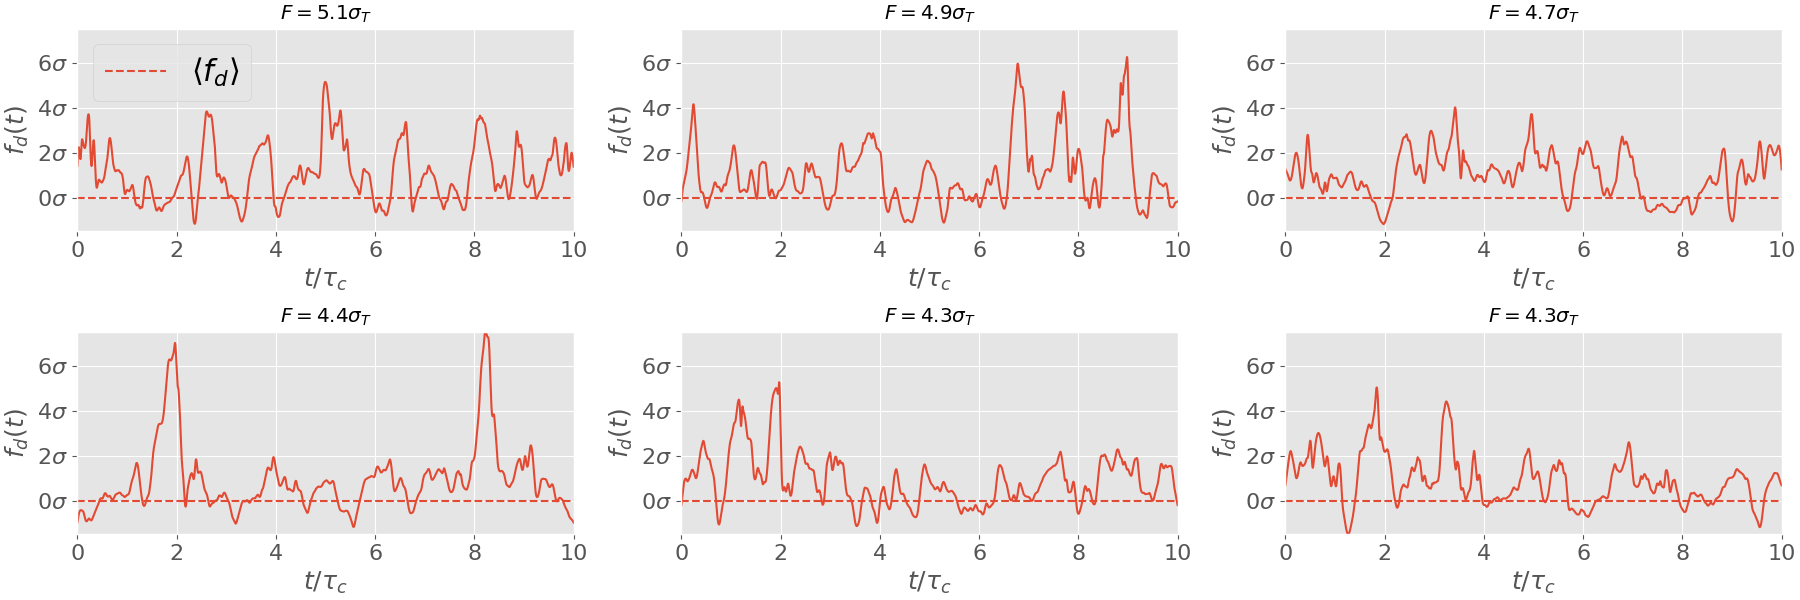
\includegraphics[width=\linewidth]{timeseries_extrms_AVG/timeseries_extrms_AVG}
	\caption{Instantaneous drag signals $f_d(t)$ corresponding to the highest fluctuations of the averaged  drag $F_T$ with a time window $T = 10 \tau_c$;  $\sigma$ and $\sigma_T$ denote the standard deviations of the instantaneous and averaged drag, respectively.}
	\label{fig:extreme_avg}
\end{figure}


% motivation
%
%In section~\ref{sec:instantaneous_drag}, we discussed the phenomenology of rare events corresponding to extremely high values of the drag acting on the square obstacle mounted in the flow described in section~\ref{sec:test_flow}. In particular, it was pointed out that such extreme drag fluctuations have a lifetime of, roughly, one correlation time $\tau_c$.

%We discussed previously the phenomenology of extreme fluctuations of the \emph{instantaneous} drag and pointed out that the time scale associated with the development of such event is of the order of the sweeping time of the flow past the obstacle $\tau_c$. 
We discussed previously the phenomenology of extreme fluctuations of the \emph{instantaneous} drag, and identified the sweeping time of the flow past the obstacle as the characteristic lifetime of these events. 
%
In applications, this duration may be much smaller than the response time of the material structure subject to these fluctuations, justifying a practical interest in the averaged (in time) drag force. 
% Consider for instance the interaction of a deformable structure with a turbulent flow: the typical response time may be much larger than the lifetime of drag fluctuations.
%
% definition
%
Therefore, a relevant observable is the \textit{time-averaged} drag defined as
\begin{equation}
  \label{eq:def_time_averaged_drag}
  F_T(t) = \frac{1}{T}\int_t^{t+T} f_d(t) \mathrm{d}t,
\end{equation}
where $f_d(t)$ denotes the instantaneous drag and $T$ is the investigated timescale (response time). Relevant values of $T$ are application dependant. We shall consider $T=10\tau_c$ in the following.

%
During a time interval $[t;t+T]$, a fluctuation of $F_T(t)$ may be roughly viewed as the overall contribution of  $T / \tau_c$ independent fluctuations of the {instantaneous} drag $f_d$.  
% phenomenology
%
% What is the phenomenology leading to extreme values of $F_T(t)$ ?
It is thus legitimate to ask whether a large value of the averaged drag results from a single outstanding fluctuation of the instantaneous drag (case (1)),  or from  an unusual succession of moderate positive fluctuations (case (2)). 
%
%
%The averaged drag signal $\{F_T(t)\}_{0 \leq t \leq T_{tot}-T}$ is obtained by filtering in time the instantaneous drag signal $f_d(t)$. 
In the same way as in section \ref{sec:extreme_extraction}, one can identify extreme fluctuations of $F_T$ exceeding some fixed threshold $a$, and sample a set of extreme events.
By taking $a=5.2\sigma_T$ with $\sigma_T$ being the standard deviation of $F_T$, $84$ independent extreme events have been selected.


% neither case (1) nor case (2)
%
Fig.~\ref{fig:extreme_avg} displays the time-series $\{f_d(t)\}_{t^{\star} \leq t \leq t^{\star}+T}$ for several extreme fluctuations of $F_T$ occurring at $t=t^\star$.
It is found that extreme fluctuations of the time-averaged drag can neither be reduced to case (1) nor case (2). 
Indeed, both cases are equally featured in Fig.~\ref{fig:extreme_avg}.  Very large value of the averaged-drag results from either a very large fluctuation, or a significant succession of moderate (positive) fluctuations of the instantaneous drag.
%
% theoretical explanation
%
This observation can be related to the exponential shape of the tail of the \ac{pdf} describing extreme positive drag fluctuations. 
Indeed, let $X$ be a random variable with a \ac{pdf} $\mathbb{P}(X)$ and a standard deviation $\sigma_X$.
Considering an extreme positive value of $S_N=\sum_{n=1}^{N}X_n$, the probability $p_1$ (resp. $p_2$) of case (1) (resp. case (2)) writes   
\begin{equation}
  \label{eq:indep}
  p_{1}  \left(\sum_{n=1}^{N} X_n = S_N\right) \propto \mathbb{P} \left({S_N}/{N} \right)^{N} \quad \text{and} \quad p_{2}  \left(\sum_{n=1}^{N} X_n= S_N\right) \propto \mathbb{P}(S_N)  
\end{equation}
If $\mathbb{P}$ has an exponential positive tail, \textit{i.e.} $\mathbb{P}(X=x) \underset{x \gg \sigma_X}{\propto} e^{-\lambda x}$, both cases (1) and (2) have equivalent probabilities provided that the average $a=S_N/N$ is very large:
\begin{equation}
  \frac{p_{2}}{p_{1}} \underset{a\to \infty}{\to} \left(e^{\lambda a }\right)^{N} e^{-\lambda a N} = 1
  \label{eq:ratio_exp}
\end{equation}
The observation is therefore well supported theoretically.
See~\cite{lestang2019JSTAT} for further details.


\section{Rare-event algorithms}
\label{sec:rare_events_algorithms}
% limitation of direct sampling
%
In the limit of very rare events and complex dynamics such as turbulent flows in industrial or environmental domains, the computational cost of  direct sampling becomes prohibitive. According to Eq.~\eqref{eq:return_time}, the return time of fluctuations $f_d \geq a$ scales as $r(a) \propto e^{l a}$.
As a consequence, the computational cost required to sample events of amplitude $f_d \geq a$ through brute-force sampling diverges exponentially as $e^{l a}$.
%% objective
% In this section we discuss the application of \textit{rare event algorithms} to the numerical sampling of extreme drag forces on immersed objects, on the example of the flow presented in section~\ref{sec:test_flow}.
The motivation behind rare-events algorithms is to sample extreme fluctuations for a computational cost much lower than their related return times.
%
For this purpose, the \acl{ams} (\ac{ams}) and \acl{gktl} (\ac{gktl}) algorithms are considered in the following.
%
%
Both algorithms rely on an ensemble of $N$ trajectories $\{\mathbf{x}_n(t)\}_{0\leq t \leq T_a}$ with $n=1 \cdots N$.
Each $\{\mathbf{x}_n(t)\}_{0\leq t \leq T_a}$ refers to a trajectory (of duration $T_a$) of the system in phase space. In our case, the dynamical system under investigation is the flow described in section~\ref{sec:test_flow}.
%In a nutshell
Briefly, trajectories are replicated or discarded in the ensemble according to some \emph{selection rules} designed to sample rare events of some observable, \textit{e.g.} the drag, with a higher frequency.
These selection rules are such that the introduced statistical bias is known at each iteration of the algorithm.
The generated trajectories are associated with a weight, from which one is able to compute the probability and expectation values of observables. 
% These two algorithms will be detailed in the following.
% In section~\ref{sec:ams}, we highlight that sampling  extreme fluctuations of the instantaneous drag with the \ac{ams} algorithm is a difficult task.
% In section~\ref{sec:gktl}, we apply an importance sampling algorithm, the \ac{gktl} algorithm, and efficiently sample rare trajectories corresponding to extreme fluctuations of the time-averaged drag.
% As an application, we use the \ac{gktl} algorithm to compute return times of very rare drag fluctuations.


\subsection{Extreme instantaneous drag forces with the \acl{ams} algorithm}
\label{sec:ams}

\begin{figure}
  \centering
  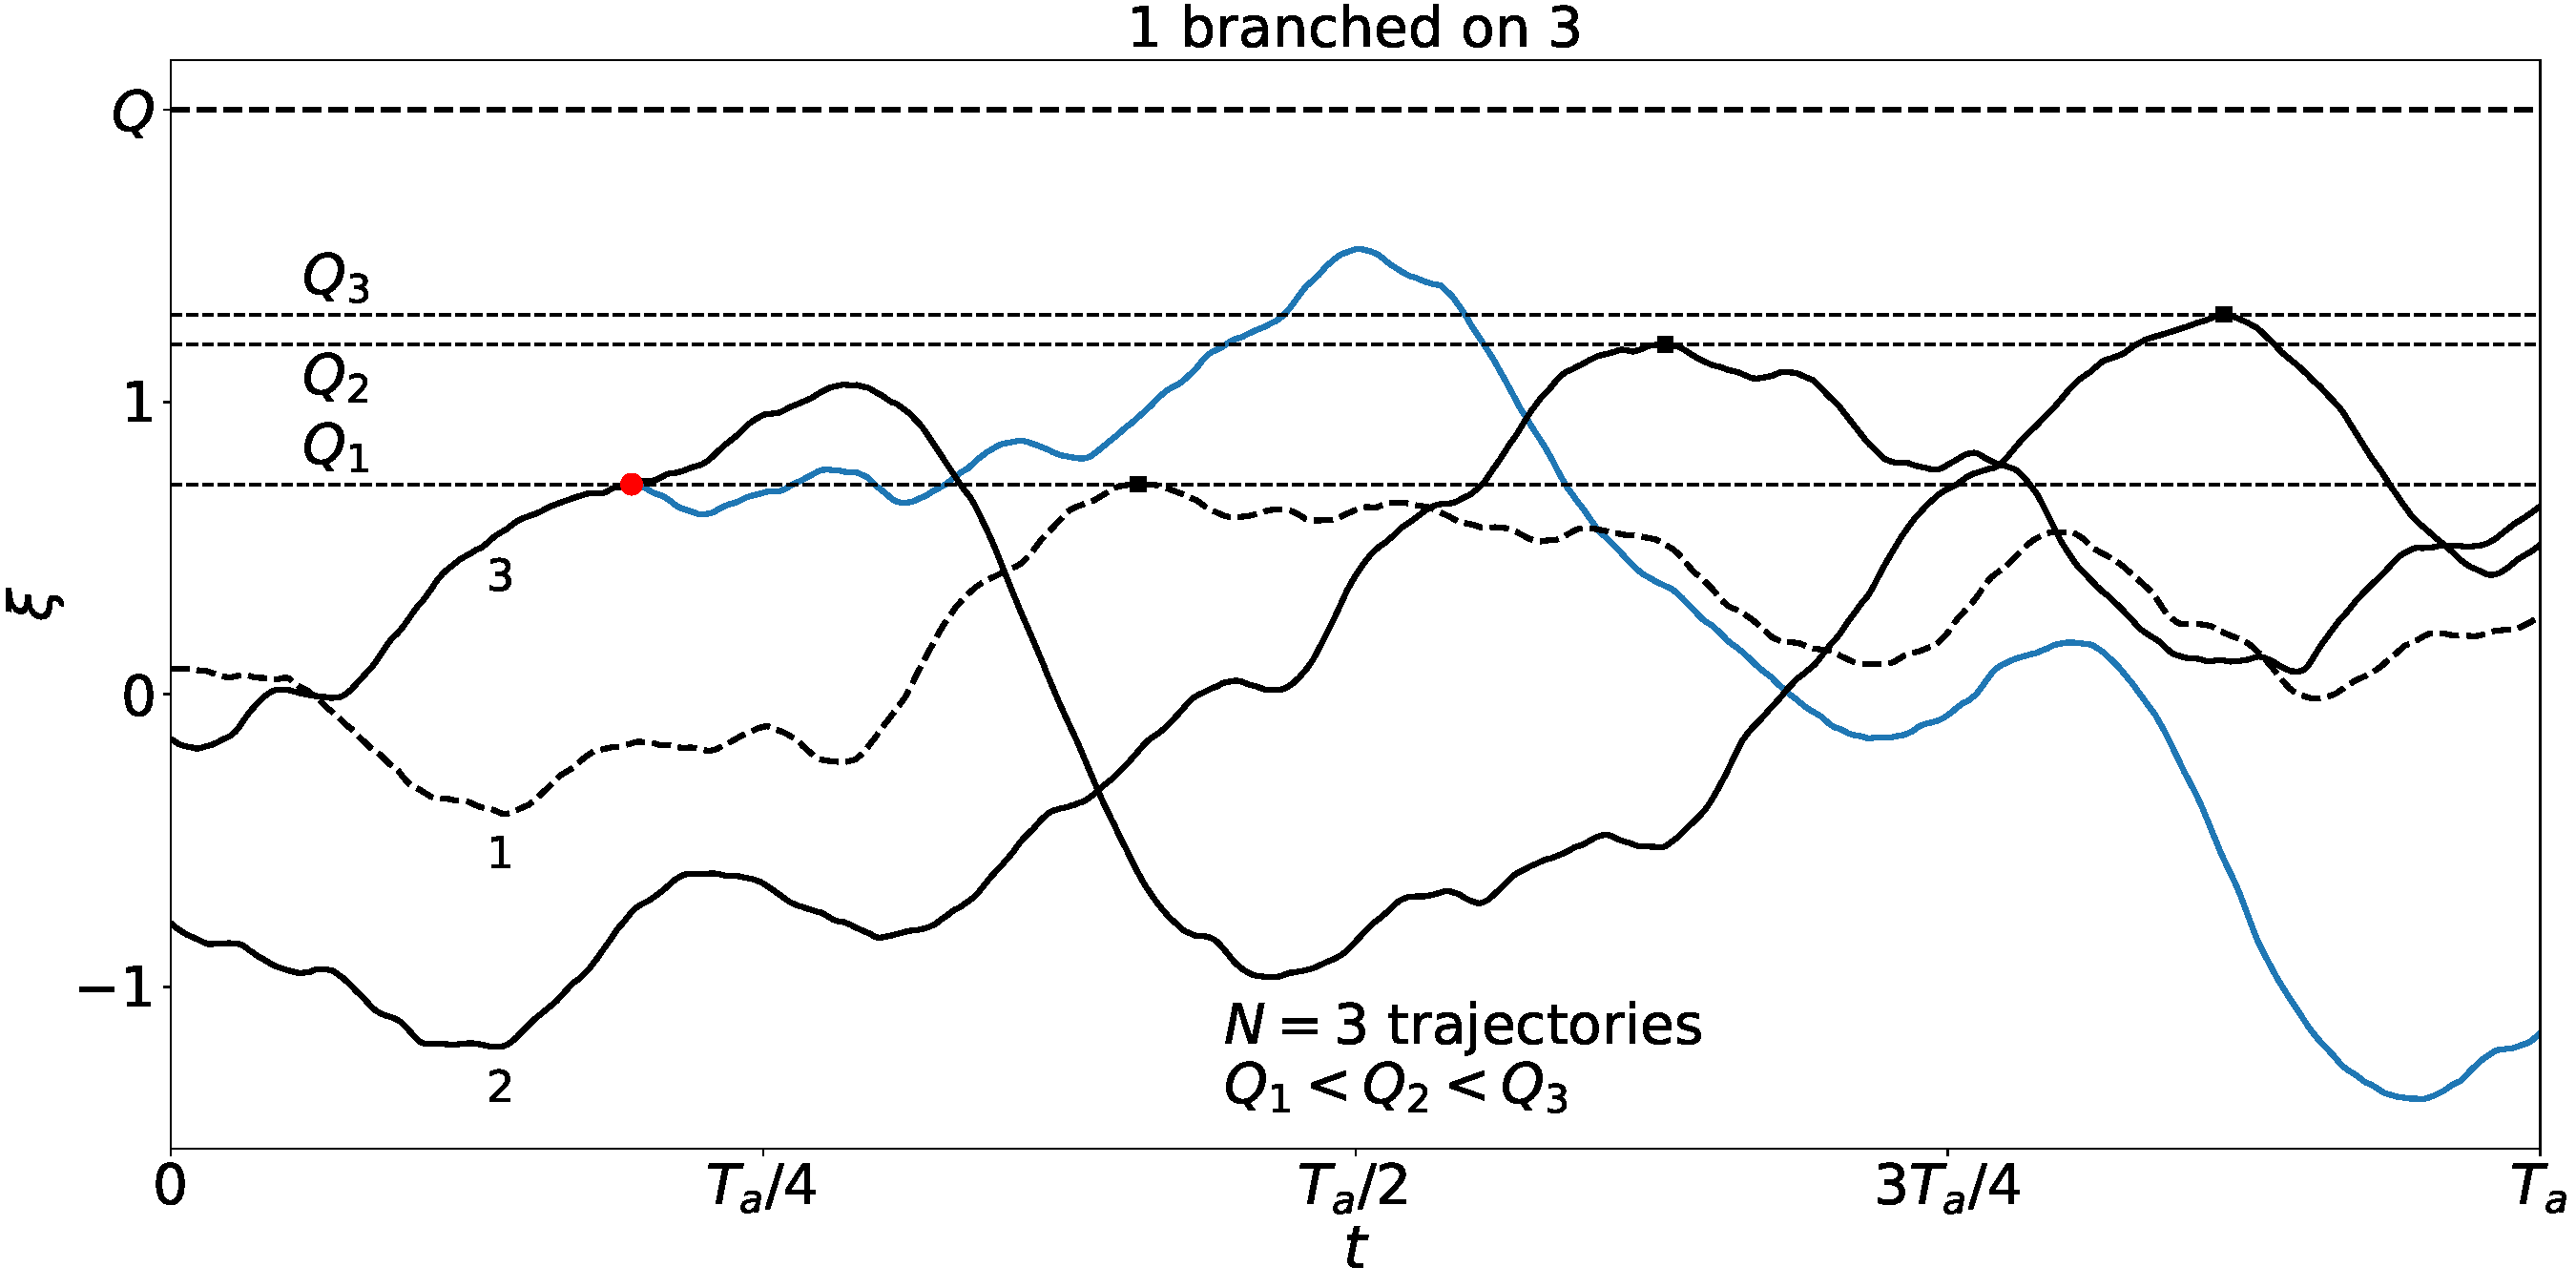
\includegraphics[width=\linewidth]{illustr_AMS/illustr_AMS}
  \caption{\label{fig:illustr_AMS} Selection-mutation procedure of the \ac{ams} algorithm with $N=3$. Lines 1, 2 and 3 represent the evolution of the score function for the current ensemble of trajectories. On the basis of their respective maximum: $Q_1$, $Q_2$ and $Q_3$, the trajectory with the lowest maximum is discarded in the ensemble (dashed line). Among the two remaining trajectories, trajectory 3 is chosen randomly and copied until it reaches the value $Q_1$. It is then simulated from the branching point to the final time $T_a$. In case of deterministic dynamics, a small perturbation is introduced at the branching to separate the trajectories. Depending on the application, this re-sampling procedure can iterated $J$ times or until all trajectories do exceed a fixed threshold $Q$.}
\end{figure}

% Introduction of AMS
%
The \acl{ams} algorithm \cite{cerou_adaptive_2007} inherits the basic ideas of {splitting algorithms} \cite{KahnHarris1951}. The sampling of a rare event is made easier by splitting the dynamical path of the system (in phase space) into 
%a sequence of events that can be sampled with a higher probability  
a sequence of short excursions \cite{glasserman_multilevel_1999,rolland_statistical_2015}.
The related selection-mutation step of this algorithm {relies on the definition of a \textit{score function} $\xi (\mathbf{x}(t),t)$}.
The operating principle is sketched in Fig.~\ref{fig:illustr_AMS}.
%
% As already mentioned in the introduction, the \ac{ams} has been successfully applied to a large body of problems for the past ten years. 
%
% Over the past ten years the \ac{ams} has been successfully applied to a large body of problems, including the computation of the dissociation time of biomolecules~\cite{teo_adaptive_2016} or the simulation of rare relaminarizations in a stochastic model of wall turbulence~\cite{rolland_extremely_2018}.
%
% Quick description of TAMS
%
Iterations of the algorithm consist in discarding the trajectories with the lowest maxima of the score function during the time interval $0\leq t \leq T_a$.
Discarded trajectories are re-sampled according to the remaining trajectories.
See~\cite{cerou2019adaptive} for a review of the \ac{ams} algorithm, its history and applications.
For recent applications of the \ac{ams} in the context of fluid turbulence, see \cite{bouchet2019rare,rolland_extremely_2018}.
{Let us mention that we use a specific form of the \ac{ams}, in which trajectories have a fixed duration $T_a$.
It can however be formulated in terms of the ``classical \ac{ams}''~\cite{lestang_computing_2018}. Next results are therefore not limited to this particular variant.}



\subsubsection{Illustration of the \ac{ams} on a simple case: the \acl{ou} process}
\label{sec:ams_ou}
% Example: OU process
\begin{figure}
  \centering
  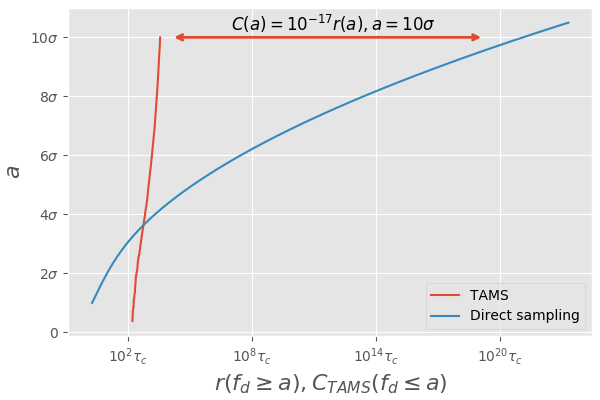
\includegraphics[width=.7\linewidth]{AMS_OU/AMS_OU.png}
    \caption{Efficiency of the \ac{tams} algorithm with respect to direct sampling in the case of an Ornstein-Uhlenbeck process \cite{lestang_computing_2018}. The red line represents the evolution of the maximum obtained from re-sampled trajectories as a function of the computational cost $C_{TAMS}$. The blue line is the analytical solution for the return time of amplitude $a$.}
  \label{fig:comparaison_temps_de_retour}
\end{figure}
Fluid dynamics is temporarily left aside and a one-dimensional \acl{ou} process is considered:
\begin{equation}
  \label{eq:ou}
  \dot{x} = -x + \eta (t),
\end{equation}
where $\eta$ is a Gaussian noise with $\langle \eta(t)\eta(t-t')\rangle = \delta(t-t')$.
This basic stochastic process will allow us to highlight differences with fluid dynamics.


The \ac{ams} is applied  to a set of $N=32$ trajectories $\{x_n(t)\}_{0\leq t \leq T_a}$ with $T_a=5\tau_c$.
Let us note that the correlation time is $\tau_c = 1$ for the process defined by Eq.~\eqref{eq:ou}.
Our objective is to sample fluctuations $x\geq a$ with $a$ being very large compared to the typical values of $x$.
The score function is simply $x(t)$ and a single trajectory is re-sampled at each iteration.
%
%Let $a_j$ be the maximum of the re-sampled trajectory at iteration $j$.
%
The computational cost of the algorithm after $J$ iterations is therefore related to the simulation of the $N$ initial trajectories and the re-sampling of $J$ trajectories.
Fig.~\ref{fig:comparaison_temps_de_retour} compares the computational cost of the \ac{ams} algorithm with that of a direct sampling. 
In the latter, the typical computational cost is simply the return time $r(a)$.
Obviously, the successive re-samplings of the \ac{ams} algorithm lead rapidly to trajectories exhibiting extreme fluctuations.
For large $a$, the computational cost is many orders of magnitude lower than that obtained by direct sampling.

Undoubtedly, the \acl{ou} process has oversimplified dynamics to showcase the efficiency of the \ac{ams} algorithm.
The state space is one-dimensional and the choice of the score function is straightforward: It is $x$ itself.
In addition, the noise term in Eq.~\eqref{eq:ou} has no correlation in time, which implies that newly generated trajectories quickly separate from their parents. Such favorable features do no a priori persist in the case of fluid dynamics.


\subsubsection{The \ac{ams} for extreme drag fluctuations}
\label{sec:ams_drag}

\begin{figure}
	\centering
	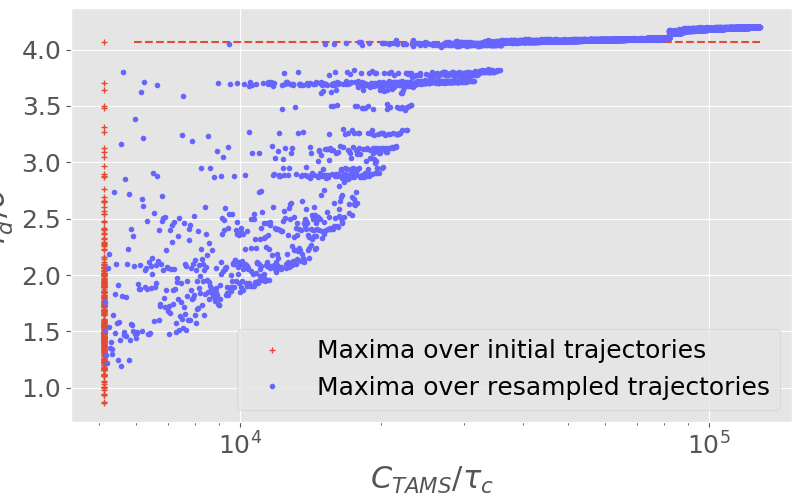
\includegraphics[width=.7\linewidth]{AMS_drag_resampling/AMS_drag_resampling.png}
	\caption{\label{fig:AMS_drag_resampling} Maximum of the instantaneous drag throughout the re-sampled trajectories as a function of the corresponding computational cost $C_{TAMS}$. The \ac{ams} is unable to efficiently sample rare trajectories associated to drag fluctuations higher than the largest fluctuation already captured in the initial ensemble.}
\end{figure}


% Application to instantaneous drag
%
% Can the \ac{ams} algorithm achieve similar performance when applied to complex chaotic dynamics, such as turbulent flows around objects ?
% To answer this question, we consider again the two-dimensional test flow introduced in section~\ref{sec:test_flow}.
%
Our aim is now to use the \ac{ams} algorithm to sample flow evolutions that exhibit extreme fluctuations of the drag $f_d$ acting on the square obstacle.
In contrast with the \acl{ou} process, the phase space is here highly-dimensional with intrinsically chaotic dynamics.
In that situation, the choice of the score function $\xi (\mathbf{x}(t),t)$ is no longer straightforward.
However, a natural simple choice for which we have opted, is $\xi (\mathbf{x}(t),t) = f_d(t)$. 
%
{Let us also stress that the dynamics is here deterministic.
Therefore, randomness must be artificially introduced for the re-sampling procedure to be effective, \textit{i.e.} to generate new trajectories associated to larger drag fluctuations.
In practice, a small perturbation in the state of the flow has been introduced at the branching points (see Fig.~\ref{fig:illustr_AMS} and~\cite{wouters2016rare}).
%
Due to the chaotic behavior of the flow, re-sampled trajectories then sparate from their parents.
% The timescale over which two trajectories separate due to an infinitesimal perturbation is known as the \textit{Lyapunov timescale}. It is denoted $\tau_L$ in the remainder of this paper.
We assume that this perturbation at branching times has a negligible impact on the statistical properties of the sampled rare events.
The validity of this assumption has been tested by performing a long simulation of the dynamics and by regularly perturbing the flow.
It was checked that the obtained statistics of the drag were consistent with the statistics computed from the (unperturbed) control simulation described in section~\ref{sec:pdfs}.}
%\EL{Freddy: provide reference for Lyapunov timescale. \#12}


% application
%
The \ac{ams} algorithm is applied to $N=256$ trajectories of duration $T_a = 20\tau_c$.
%
Fig.~\ref{fig:AMS_drag_resampling} displays the maximum drag achieved by the re-sampled trajectories as a function of the computational cost, similarly to Fig.~\ref{fig:comparaison_temps_de_retour}.
%
%
The distribution of the maximal drag for the \textit{initial} trajectories is also shown.
After a few iterations, the trajectories with the lowest maxima of the score function are discarded and new trajectories with higher maxima are re-sampled.
These maxima are depicted by the stars in Fig~\ref{fig:AMS_drag_resampling}.
Importantly, one can observe that the re-sampled trajectories never exceed the amplitude of the highest maximum already attained in the initial set of trajectories. This obviously contrasts with the case of the \acl{ou} process.
%(see Fig.~\ref{fig:comparaison_temps_de_retour}). 


\begin{figure}
  \centering
  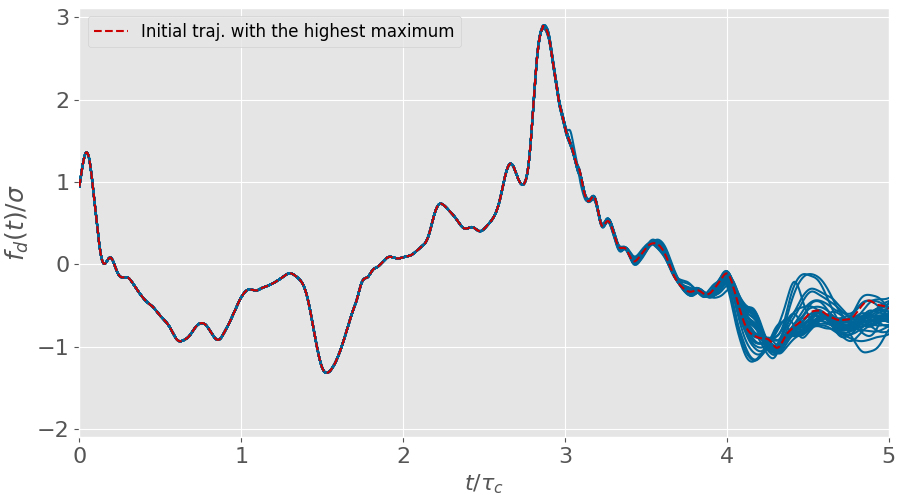
\includegraphics[width=.7\linewidth]{AMS_drag_trajectories/AMS_drag_trajectories.png}
  \caption{\label{fig:AMS_drag_trajectories} Ensemble of $N = 32$ trajectories after $181$ iterations of the selection-mutation procedure. In this experiment, the \ac{ams} algorithm is used with the instantaneous drag $f_d(t)$ as score function. Each trajectory has a duration $T_a = 5\tau_c$ (correlation time of the drag).
  The \ac{ams} fails to efficiently sample rare trajectories. All trajectories are eventually re-sampled from the same trajectory displaying the highest maximum in the initial ensemble.}
\end{figure}

%pitfall
%
Fig.~\ref{fig:AMS_drag_trajectories} displays the ensemble of trajectories after many iterations of the \ac{ams} re-sampling procedure. 
%
Let us mention that for the sake of simplicity, the trajectory of the system is here abusively associated with the time evolution of the observed drag.  
%
Interestingly, all trajectories ultimately originate from one unique initial trajectory. 
%
This feature may be explained as follows.
It takes a certain time $\tau_L$ (called Liapunov's timescale) before a re-sampled trajectory separates from its parent. In our situation, this ``memory effect'' originates from the fact that the score function is of dimension smaller (here 1) than the dimension of the phase space (very large for this fluid dynamics problem). 
%
We observe in Fig.~\ref{fig:AMS_drag_trajectories} that the duration of extreme drag fluctuations, $\tau_c$, is much shorter than the Lyapunov's timescale $\tau_L$.
As a consequence, the re-sampling of a trajectory branched close to $t=t^{\star}$ (when the maximum drag occurs) cannot lead to larger values at $t^{\star} \leq t \leq t^{\star}+\tau_L$.
For $t - t^{\star} >\tau_L$, the drag process has lost the memory of the drag fluctuations on which the re-sampling was based and, therefore, the probability of observing a new extreme fluctuation is also very low.
%

The difference between the typical duration of drag fluctuations $\tau_c$ and the Lyapunov timescale $\tau_L$ may be heuristically associated with the \emph{turbulence rate} of the flow.
%
As discussed previously, the duration of extreme fluctuations of the drag are closely related to the sweeping time of the flow past the obstacle, and consequently to the mean-flow velocity $U$. On the contrary, the Lyapunov timescale is rather associated with the intrinsic evolution of turbulent fluctuations in the reference frame of the mean flow, \textit{i.e.} with the fluctuating velocity $u_{rms}$. The ratio $u_{rms}/U$ (turbulence rate) is much lower than one in our case of grid-generated turbulence, which implies that $\tau_L \gtrsim \tau_c$.
 
%As discussed previously, extreme fluctuations of the drag $f_d$ have a lifetime of length roughly $\tau_c$.  Fluid structures responsible for a particular value of the drag on the obstacle at a time $t^{\star}$ are swept away by the mean flow over a timescale $\tau_c$, shorter than the time it takes for trajectories to separate, \textit{i.e} the Lyapunov timescale. 


% perspectives
%
In summary, it appears that a straightforward application of the \ac{ams} algorithm with the score function being the drag itself, does not allow us to efficiently sample extreme fluctuations.
%
Retrospectively, there is \textit{a priori} no reason for the drag itself to be a good indicator of how likely next drag fluctuations will develop.
On the other hand, finding a better score function would require a precise qualitative understanding of the flow scenario leading to extreme events.
%which is certainly beyond the phenomenological description developed in section~\ref{sec:dynamical_aspects}.
%
%Furthermore, such ``tuning'' is problem dependent.
%
A possible line of improvement might be to explicitly account for ``the correlation time of the observable being smaller than the Lyapunov time of the system'' by re-sampling the trajectories at a Lyapunov time {before} the maximum is reached. That way, new events associated to higher fluctuations may have the opportunity to develop.
However, such modification of the procedure must be implemented with care especially in order to preserve the mathematical properties of the algorithm, \emph{e.g} the evaluation of the statistical bias .
% 

\subsection{Importance sampling of extreme time-averaged drag forces with the \acl{gktl} algorithm}
\label{sec:gktl}
The sampling of extreme fluctuations of the time-averaged drag $F_T$ is now examined.
The \ac{ams} algorithm could be used in the same way as before
%in section~\ref{sec:ams_drag} \textit{i.e.} 
by taking the time-averaged observable itself as the score function.
However, this would lead to similar unsatisfactory results.
% the re-sampling fails to efficiently generate new higher fluctuations of $F_T$.
%
For a time-averaged observable,  an alternative approach is provided by the \acf{gktl} algorithm \cite{giardina_direct_2006,tailleur_probing_2007,giardina_simulating_2011}.
%
Similarly to the \ac{ams} algorithm, the \ac{gktl} algorithm relies on the simulation of an ensemble of trajectories.
% In this case, however, the trajectories interact dynamically. 
%
At regular time intervals, some elements of the ensemble are killed and others are cloned according to a weight that depends on the history of the replica.
%
The weights are chosen so that, after several iterations of the algorithm, the trajectories in the ensemble are distributed according to a biased probability distribution that favors trajectories related to large values of the observable.
%
The \ac{gktl} algorithm belongs to a family of algorithms called ``go with the winners'' \cite{aldous1994go,grassberger2002go}.
{Similar ideas have already been applied in a wide range of fields such as polymer physics~\cite{grassberger1998perm}, out of equilibrium statistical physics~\cite{PhysRevLett.118.115702}, computer science~\cite{aldous1994go}, dynamical systems~\cite{tailleur_probing_2007}, quantum mechanics~\cite{intro_DMC_kosztin}.}
The application of a go-with-the-winners approach to the computation of large deviations in non-equilibrium systems has first been proposed in 2006 \cite{giardina_direct_2006}.
Over the past ten years, it has successfully been applied to investigate rare events in both stochastic \cite{giardina_direct_2006,lecomte_numerical_2007,garrahan2007dynamical} and deterministic systems \cite{giardina_direct_2006,tailleur_probing_2007}.
% It was originally designed to compute large deviations rate functions of time-averaged dynamical observables, that describe the probability density of both typical of rare events in the limit of large
% averaging time~\cite{ref_large_dev}.
% By contrast with the \ac{ams} and \ac{ams}, the \ac{gktl} algorithm does not follow the strategy of splitting algorithms.
% Instead, it implements \textit{importance sampling}, \textit{i.e.} sampling a modified distribution that is biased towards the rare events of interest.
% The idea of importance sampling is very general and was used in many different contexts (see e.g.~\cite{Berg1992,Hartmann2002} and the general references~\cite{Bucklew2004,RubinoTuffin2009}). 
% The \ac{gktl} algorithm performs importance sampling in the space of trajectories, which is relevant for out-of-equilibrium systems.

\subsubsection{The \ac{gktl} algorithm}
\label{sec:gktl_description}
The \ac{gktl} algorithm is based on the simulation of an ensemble of $N$ trajectories $\left\{\mathbf{x}_{n}(t)\right\}_{0\leq t \leq T_a}$ with $ n =1 \cdots N$ starting from independent random initial conditions.
%
Let us consider a real-valued observable of interest $A(\mathbf{x}(t))$, {\emph{e.g.} the drag $f_d(t)$}, and introduce a cloning period $\tau$.
%
At time instants $t_{i}=i\tau$ with $i=1,~2,~...,~T_{a}/\tau$ ($T_{a}$ is a multiple of $\tau$) a weight $W_{n}^{i}$ is assigned to each trajectory. This weight is defined ($t_0=0$) by
%
\begin{equation}
W_{n}^{i}=\frac{e^{k\intop_{t_{i-1}}^{t_{i}}A(\mathbf{x}_{n}(t))dt}}{R_{i}}\quad \mbox{with the normalisation factor} \quad R_{i}=\frac{1}{N}\sum_{n=1}^{N}e^{k\int_{t_{i-1}}^{t_{i}}A(\mathbf{x}_{n}(t))dt}
\label{eq:Weight}
\end{equation}
so that $\sum_{n=1}^N W_n^i = N$.
%
%
{The weights $\{W_{n}^{i}\}_{n=1\cdots N}$ determine how many copies of each trajectory are made at time $t=t_i$. The parameter $k$ characterizes the amplitude of the statistical bias involved in the algorithm (see Fig.~\ref{fig:IS_GKTL}). For more information about the practical implementation of the algorithm, the interested reader can refer to~\cite{brewer2018efficient, lestang:tel-01974316}}.
The application of this re-sampling at each step $t_i$ eventually leads to a biased sampling in the trajectory space; the trajectories corresponding to extreme values of $\int_{0}^{T_a}A(\mathbf{x}_{n}(t))dt$ have a higher probability.
%
The sampled biased distribution writes
%
\begin{align}
\mathbb{P}_{k}\left(\left\{ \mathbf{X}(t)\right\} _{0\leq t\leq T_{a}}=\left\{ \mathbf{x}(t)\right\} _{0\leq t\leq T_{a}}\right) &\underset{N\rightarrow\infty}{\sim} \frac{e^{k\int_{0}^{T_{a}}A(\mathbf{x}(t))dt}}{Z(k,T_a)}\mathbb{\mathbb{P}}_{0}\left(\left\{ \mathbf{X}(t)\right\} _{0\leq t\leq T_{a}}=\left\{ \mathbf{x}(t)\right\} _{0\leq t\leq T_{a}}\right),
\label{eq:Biased_Path_Approximation}
\end{align}
where
$\mathbb{P}_{0}\left(\left\{ \mathbf{X}(t)\right\} _{0\leq t\leq T_{a}} = \left\{ \mathbf{x}(t)\right\} _{0\leq t\leq T_{a}}\right)$ 
refers formally to the probability of observing the trajectory 
$\left\{ \mathbf{x}(t)\right\} _{0\leq t\leq T_{a}}$.
The normalisation factor is given by $Z(k,T_a)=\prod_{i=1}^{T_a/\tau}R_i$.
%
One can mention that
\begin{equation}
  \label{eq:mean_field}
  Z(k,T_a) \underset{N\to \infty}{\sim} \mathbb{E}_0\left[e^{k\int_{0}^{T_{a}}A(\mathbf{X}(t))dt}\right],
\end{equation}
with $\mathbb{E}_{0}$ being the expectation value with respect to the
distribution $\mathbb{P}_{0}$.
This result relies on the \textit{mean-field approximation}

\begin{equation}
R_{i}=\frac{1}{N}\sum_{n=1}^{N}e^{k\int_{t_{i-1}}^{t_{i}}A(\mathbf{X}_{n}(t))dt}\underset{N\rightarrow\infty}{\sim} Z(k,t_i)= \mathbb{E}_{i}\left[e^{k\int_{t_{i-1}}^{t_{i}}A(\mathbf{X}(t))dt}\right],
\label{eq:Mean_Field_Approximation}
\end{equation}
where $\mathbb{E}_{i}[.]$ denote the expectation value with respect to the biased distribution $\mathbb{P}_k^{(i)}$ obtained after $i$ cloning steps.
The typical relative error related to this approximation can be shown to be of order $1/\sqrt{N}$ for a family of rare-event algorithms including the \ac{gktl} algorithm~\cite{DelMoralBook,DelMoral2013}.
%
Rejected trajectories are discarded from the statistics.
Eventually, an effective ensemble of $N$ trajectories of duration $T_{a}$ is obtained, distributed according to $\mathbb{P}_{k}$.


A key feature of the \ac{gktl} algorithm is that the sampling procedure does not involve any alteration of the dynamics. All trajectories in the resampled ensemble are solutions of the original dynamical. 
%This is true for stochastic dynamics.
{Nevertheless, it should be noted that a (small) random perturbation is introduced in the cloning procedure to allow the trajectories of two clones to separate. 
As for the \ac{ams} algorithm, it is assumed that this perturbation does not (notably) affect the statistics of the sampled trajectories.}
% 
%However, similarly to the case of \ac{ams}, randomness must be artificially introduced for the cloning procedure to be effective for deterministic dynamics in order to separate the clones. We have proceeded in the same way as as described in section~\ref{sec:ams_drag}.
%
%
Eventually, the sampled trajectories obtained with the \ac{gktl} algorithm can be used to compute the statistical properties of any observable with respect to the distribution $\mathbb{P}_{0}$ from the distribution $\mathbb{P}_{k}$ by using Eq.~\eqref{eq:Biased_Path_Approximation}.
%


\subsubsection{Application of the \ac{gktl} algorithm to extreme fluctuations of the time-averaged drag}
\label{sec:gktl_drag}

\begin{figure}
	\centering
	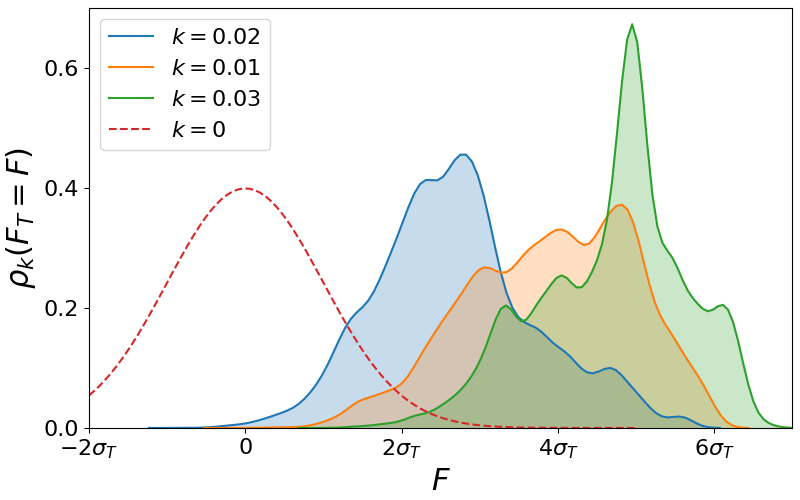
\includegraphics[width=0.7\linewidth]{IS_GKTL/IS_GKTL}
	\caption{\label{fig:IS_GKTL} Rare-event sampling of the (zero-mean) time-averaged drag $\tilde F_T = F_T - \overline{F_T}$ with $T=10\tau_c$; $\tau_c$ is the correlation time of the instantaneous drag. The shaded \ac{pdf}s are estimated from the biased ensemble resulting from the \ac{gktl} algorithm applied to $16384$ trajectories of duration $T_a=T$ with the cloning period $\tau=\tau_c/2$.
	The dashed line refers to the unbiased \ac{pdf} of $\tilde F_T$, \textit{i.e.} obtained from direct sampling or with $k=0$ (no bias) in the \ac{gktl} algorithm.
}
\end{figure}

The application of the \ac{gktl} algorithm is now considered for the flow dynamics introduced in section~\ref{sec:test_flow}. The purpose is to sample trajectories with extreme fluctuations of the \textit{time-averaged} drag, $F_T$. {Referring to the previous notations, $A(\mathbf{x}(t))=f_d(t)$ is our observable of interest and the duration $T_a$ of each trajectory corresponds to the period of averaging of the drag, \emph{i.e.} $T_a=T$.}    

% Choice of parameters and perturbation
The computational cost $C_{{gktl}}$ depends on both the duration of each trajectory and the number of trajectories: $C_{gktl} = N \times T_a$.
We have taken $N=16384$ and $T_a = 10\tau_c$ which yields $C_{gktl} \approx 1.6 \times 10^5 \tau_c$. The choice of the cloning period $\tau$ is important in practise.
A  cloning period too-short can result in a loss of information if the clones do not separate from their parents between two cloning steps. On the contrary, choosing $\tau \gg \tau_c$ may result in insufficient cloning steps to allow for efficient importance sampling.
As a result, a safe rule of thumb is to take $\tau$ of the order of $\tau_c$.
In the following experiments, $\tau = \tau_c /2$. 
%



Three numerical experiments corresponding to three different values of the parameter $k$ have been carried out.
%
%
%Let us remark that the value of $k$ should be chosen empirically unless a \textit{large deviation regime} $T_a \to \infty$ is verified  \cite{touchette_large_2009}.
%In the latter case, the parameter $k$ can be related to the typical amplitude of the sampled fluctuations through the Gartner-Ellis theorem \cite{touchette_large_2009}.
%
%
Fig.~\ref{fig:IS_GKTL} shows the estimate of the biased \ac{pdf}s of the (zero-mean) time-averaged drag $\tilde F_T \equiv F_T - \overline{F_T}$, \emph{i.e}
\begin{equation}
  \label{eq:estimate_biased_measure}
  \rho_k(F) 
  %= \mathbb{E}_{\mathbb{P}_k}[\delta(\tilde F_T(\{\mathbf{x}\}_{0\leq t \leq T_a})-F)]
  \approx \frac{1}{N}\sum_{j=1}^{N}\delta(\tilde F_{T}(\{\mathbf{x}_j\}_{0\leq t \leq T_a}) - F)
\end{equation}
in addition to the unbiased \ac{pdf} based on the control run.
As expected, the biased PDFs obtained by applying the \ac{gktl} algorithm are centered around increasing fluctuations with the parameter $k$.
%Note that the unbiased \ac{pdf} could also be estimated using the \ac{gktl} algorithm with $k=0$.
%
% limitations
%
Nevertheless, let us mention that for a fixed number of trajectories, there is necessarily an upper limit $k_{max}$ over which the finite number of trajectories becomes detrimental to the efficiency and accuracy of the selection procedure.
%
For $k \gtrsim k_{max}$, the re-sampling relies only on a small number of ``independent trajectories'' and most of the trajectories (in the biased ensemble) overlap. 
This effect is highlighted in Fig.~\ref{fig:IS_GKTL} where the biased \ac{pdf} corresponding to $k=0.03$ is artificially peaked.
%
Such a finite-size effect is expected to gradually increase as the bias amplitude  $k$ is increased.
%
An important question concerning the application of the \ac{gktl} algorithm is therefore that of the dependence of $k_{max}$ on the ensemble size $N$. This issue is addressed in recent studies \cite{nemoto2017finite,Guevara_Hidalgo_2018}.
%
% how to assess the value of k_max ?
In the present work, the order of magnitude of $k_{max}$ has been estimated \emph{empirically} by evaluating the diversity of the trajectories in the biased ensemble.
This diversity has been monitored at each selection step of the algorithm by calculating the proportion of trajectories sharing the same ancestor trajectory.

\begin{table}
	\centering
	\begin{tabular}{|l|c|c|c|c|c|}
		\hline
		& $\sigma$ & $2\sigma$ & $3\sigma$ & $4\sigma$ & $5\sigma$ \\
		\hline
		$k=0.02$ & ~1594~ & ~799~ & ~155~ & 22 & 0  \\ 
		\hline
		$k=0.025~$ & 1019 & 834 & 521 & 198 & 27  \\ 
		\hline
		$k=0.03$ & 539 & 510 & 391 & 205 & 36  \\ 
		\hline
		${N}_{brute-force}$ & 2599 & 37 & 22 & ~0.5~ & ~0.005~ \\
		\hline
	\end{tabular}
	\caption{Number of fluctuations $F_{T} \geq a$ with a=$\sigma,~2\sigma,$ etc. captured in the biased ensemble for $k=0.02,~0.025$ and $0.03$.
		Note that trajectories that overlap for more than half of their duration are counted as only one.
		${N}_{brute-force}$ is the number of fluctuations expected from the direct sampling of $N$ independent realizations of $F_{T}$.}
	\label{tbl:nbTraj_tbl}
\end{table}

% Comparisons with direct sampling
%
The efficiency of the \ac{gktl} algorithm is now assessed with respect to direct sampling. 
Table~\ref{tbl:nbTraj_tbl} indicates the number of trajectories that correspond to a time-averaged drag $\tilde{F}_{T} \geq a$ for different values of the bias parameter $k$.
Note that trajectories that overlap for more than half of their duration are counted  as only one.
%\footnote{Trajectories that overlap over an interval $[O;t]$ with $t\geq T_a / 2$.}
Table~\ref{tbl:nbTraj_tbl} also indicates the expected number of fluctuations obtained by simulating $N$ independent trajectories $\{F_T(t)\}_{0\leq t \leq T_a}$ without resampling.
%
%This number assumes that the values of the time-average drag $F_T$, with $T=10\tau_c$, are Gaussian distributed. This hypothesis is motivated by Fig.~\ref{fig:PDF_AVG}.
%
%\begin{figure}
%  \centering
%  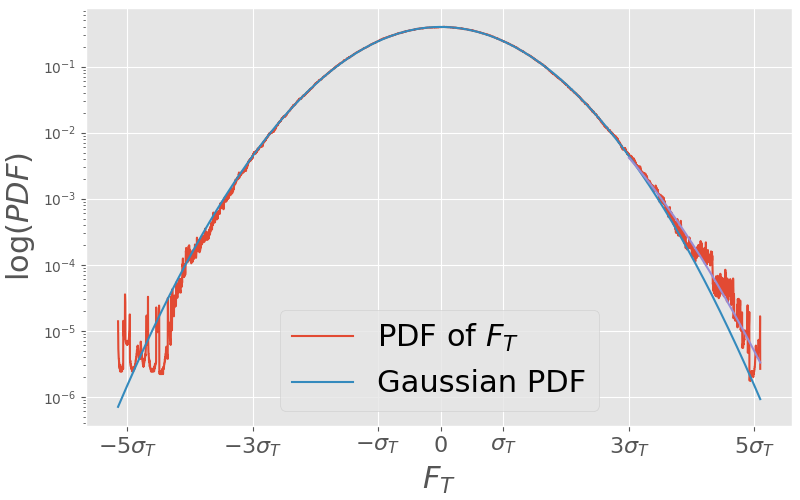
\includegraphics[width=.7\linewidth]{PDF_AVG/PDF_AVG}
%  \caption{PDF of average drag over $10\tau_c$}
%  \label{fig:PDF_AVG}
%\end{figure}
%
% Conclusion
%
We obtain that the \ac{gktl} algorithm is able to sample drag fluctuations that are far from reach by direct sampling with an equivalent computational cost.


%
% PARAGRAPHE SUIVANT INUTILE ?
%
%In section~\ref{sec:time_avg} we observed that extremely large values of the time-averaged drag can either result from a succession of rather typical---however all positive---fluctuations of the instantaneous drag $f_d$, or from a small number of extremely large fluctuations of the instantaneous drag. By selecting trajectories based on the previous average value of the drag over a duration $\tau \approx \tau_c$, the \ac{gktl} algorithm is well suited for the preferential selection of trajectories of the former kind. However, such selection strategy does not appear equally as favourable to trajectories of the latter type, for which all of the drag density is located in one or two very large fluctuations of the instantaneous drag. Further work must now investigate the nature of the sampled trajectories, and determine the amount of discrepancy concerning their respective phenomenology.



\subsubsection{Computation of return times}
\label{sec:return_times}
Statistics of extreme events can be computed from the biased ensemble by inverting Eq.~\eqref{eq:Biased_Path_Approximation}. For instance, it is possible to compute return times  for
events unreachable by a direct approach.
%(see Fig.~\ref{fig:illustrate_return_time})

In the following, the \ac{gktl} algorithm is used with $N=1024$ trajectories of duration $T_a > T= 10\tau_c$.
Each trajectory in the biased ensemble results in a timeseries of the time-averaged drag
\begin{equation}
\label{eq:time_averaged}
F_T(t) = \int_{t-T}^{t}f_d(\tau)d\tau, \quad t\in [T,T_a]  
\end{equation}
and the return time of a fluctuation $F_T \geq a$ is given by~\cite{lestang_computing_2018}
\begin{equation}
r(a) = - \frac{T_a - T}{\ln (1-\mathbb{P}(F_T \geq a))}.
\end{equation}


The probability $\mathbb{P}(F_T \geq a)$ can be estimated from the biased ensemble by inverting Eq.~\eqref{eq:Biased_Path_Approximation}
\begin{equation}
\mathbb{P}(f_d \geq a) \approx \frac{1}{N}\sum_{j=1}^{N}e^{T_a \lambda(k)}e^{k \int_{0}^{T_a}f_d(t)dt}s_j(a)
\end{equation}
with $s_j(a) = 1$ if $\max_{T\leq t \leq T_a}[F_T^{(j)}] \geq a$ and $s_j(a) = 0$ otherwise, \emph{i.e.} by summing the weights of the timeseries which maximum is larger than $a$.

Fig.~\ref{fig:return_times_gktl} displays the return times for extreme fluctuations of the time-averaged drag acting on the square obstacle.
The figure shows two independant estimates, obtained using different values of the bias parameter $k$.
Note that both estimates have been computed with the same computational cost $T_{tot}=N\times T_a$.
In addition, figure~\ref{fig:return_times_gktl} shows an estimate computed through direct sampling with the same computational cost, \textit{i.e.} using a timeseries of duration $T_{tot}$.
While a direct approach cannot access events with a return time greater than $T_{tot}$, the \ac{gktl} algorithm allows us for the computation of statistics for drag fluctuations having a return time several orders of magnitude above $T_{tot}$. This is  obviously a major advantage of this rare-event sampling algorithm. 

\begin{figure}
	\centering
	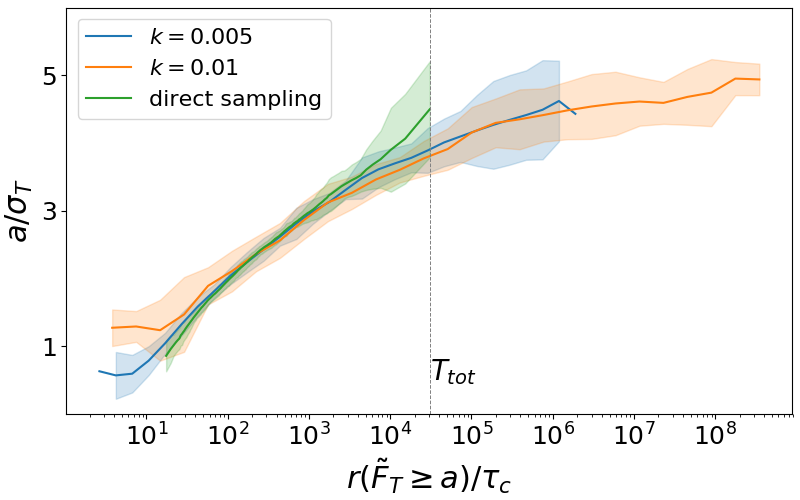
\includegraphics[width=.7\linewidth]{return_times_GKTL/return_times_GKTL}
	\caption{\label{fig:return_times_gktl} Return times for the time-averaged drag acting on the square obstacle. $\tilde{F}_T$ denotes the time-averaged drag with zero mean. The blue and read lines are obtained from the biased ensemble of trajectories generated by the \ac{gktl} algorithm with $N=1024$ and $T_a=30\tau_c$. The green line is the return times obtained from a single timeseries of duration equal to the computational cost of both \ac{gktl} experiments. Uncertainty ranges for the \ac{gktl} estimates are computed as the standard deviation over a set of 10 independent experiments. Uncertainty ranges for the direct estimation are computed as the standard deviation over a ensemble of direct estimates resulting from 60 independent timeseries.}
\end{figure}


%\subsubsection{Discussion}
%\label{sec:discussion_gktl}
%
%%
%In section~\ref{sec:time_avg} we observed that extremely large values of the time-averaged drag can either result from a succession of rather typical---however all positive---fluctuations of the instantaneous drag $f_d$, or from a small number of extremely large fluctuations of the instantaneous drag.
%By selecting trajectories based on the previous average value of the drag over a duration $\tau \approx \tau_c$, the \ac{gktl} algorithm is well suited for the preferential selection of trajectories of the former kind.
%However, such selection strategy does not appear equally as favourable to trajectories of the latter type, for which all of the drag density is located in one or two very large fluctuations of the instantaneous drag.
%Further work must now investigate the nature of the sampled trajectories, and determine the amount of discrepancy concerning their respective phenomenology.






\section{Conclusion}
\label{conlusion}
In this study, the application of two rare-event sampling algorithms has been assessed for the simulation of extreme mechanical efforts on structures immersed in a turbulent flow; a situation relevant to many industrial applications.


In a first part, we investigated the dynamics and statistics of extreme fluctuations of the drag acting on a square placed in a turbulent channel flow, in two dimensions.
By means of a long simulation of reference, we observed that such extreme events are caused by the (temporary) trapping of vorticity very close to the base of the square.
Extreme drag amplitudes do not persist over time since the mean flow eventually sweeps away the fluid structures responsible for this situation.
%
The lifetime of extreme drag fluctuations is therefore of the order of the turnover time, and the corresponding drag signal is very peaked around these extreme values.
Our long drag timeseries also reveal that the tails of the \ac{pdf} for the drag are  well described by an exponential \ac{pdf}.
This property is linked to the phenomenology of extrema of the time-averaged drag.
Especially, we observed that such extreme values for the average do not preferentially result from a small number of very large fluctuations, or an exceptional succession of moderate fluctuations that
pile up to yield an large value of the average.
Such a phenomenology is observed for stochastic processes with an exponential \ac{pdf}.

The application of rare event algorithms relies on the definition of a score function for the selection of trajectories.
%Although the dynamics itself is a black-box from the point of view of the algorithm, 
The efficiency of the algorithm depends on the choice of the score function which has to be well suited to the phenomenology of the extreme dynamics.
For complex dynamics including turbulent flows, this choice is  difficult because of the lack of characterization of rare events. These latter are expected to depend on the dynamical regime (Reynolds number), the stirring mechanism and boundary conditions of the flow. In this context, the choice of the observable itself as score function is certainly a safe fall-back option, nevertheless not optimal.
%This is, after all, our motivation for the simulation of these events.
\\
On the basis of the same two-dimensional test flow, we then applied the \ac{ams} algorithm choosing the drag itself as a score function.
In this case, our results illustrate that the selection-mutation procedure is unable to generate rare trajectories at a better rate than a direct sampling.
This can be related to the phenomenology of extreme drag fluctuations, which lifetime is shorter than the timescale over which re-sampled trajectories separate from their parent. 
%following the addition of a small perturbation in the initial conditions.
The \ac{gktl} algorithm has been applied to the sampling of trajectories displaying extreme fluctuations of the time-averaged drag.
In this case, we showed that using \ac{gktl} leads to a significant gain with respect to a direct approach, allowing for the simulation and computation of statistics for (very) rare trajectories.
The sampling of extreme time-averages is aided by the selection of trajectories displaying an exceptional succession of drag fluctuations, resulting in an extreme value of the average.
It is however unclear whether the \ac{gktl} is suited to sample trajectories for which the extreme fluctuations of the time-averaged drag results from a unique, exceptionally large drag fluctuation. This issue is postponed for future investigations.

Importantly, successful usage of the \ac{ams}, \ac{gktl} or similar algorithms for complex flows relevant to industrial or environmental situations will require coping with the fact that optimal score functions
are difficult to identify, if even possible.
A promising direction explored in current research is to take advantage of recent advances in \emph{learning methods} to optimize score functions beforehand.

\appendix*
\section{The \acl{lbm}}
\label{sec:lbm}

% details about LBM
In the LB method, the fluid is viewed as populations of particles that collide, redistribute and propagate along the different links of a discrete lattice. 
In our two-dimensional situation, the so-called D2Q9 lattice with only nine possible velocities $\{\mathbf{c_i}\}_{i=0...8}$ at each node has been adopted (see  Fig.~\ref{fig:D2Q9}).
Locally, the macroscopic flow variables (per unit volume) are recovered by summing over the densities of particles $\{f_i\}_{i=0...8}$ moving with the different velocities, i.e.
\[
\rho(\mathbf{x},t) = \sum_i f_i(\mathbf{x},t) \quad \mathrm{and}\quad \rho(\mathbf{x},t) \mathbf u(\mathbf{x},t) = \sum_i f_i(\mathbf{x},t) \mathbf{c_i}
\]
for the mass density and the fluid momentum respectively. The assumption of weak compressibility (for an ideal gas) is made so that the pressure is directly proportional to the mass density: $p = c_s^2 \rho$ where $c_s$ is interpreted as a speed of sound.  

\begin{figure}
	\centering
	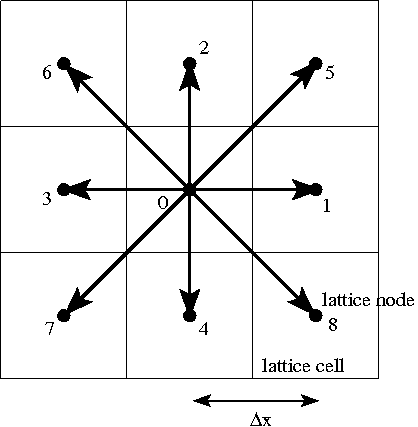
\includegraphics[width=0.3\linewidth]{D2Q9/D2Q9}
	\caption{Sketch of the D2Q9 lattice. Particles move exactly from a lattice node towards one of its nine neighbours (including the node itself) during one time step. By definition, the lattice spacing is related to the time step by $\Delta x/ \Delta t = \sqrt{3} c_s$ where $c_s$ is interpreted as a speed of sound.}
	\label{fig:D2Q9}
\end{figure}


% algo
%
The complexity of the flow emerges from the repeated application of simple rules of streaming and collision. The LB scheme advances the local densities of particles $f_i(\mathbf{x},t)$ moving with velocities $\mathbf{c}_i$  in a two-step procedure. Namely, an \emph{exact} streaming step 
\[
f_i(\mathbf{x}+\mathbf{c}_i \Delta t, t + \Delta t) = f_i^{\mathrm{out}}(\mathbf{x},t)
\]
during which particles move with their own velocity to a neighbouring node, and an instantaneous collision step
\[
f_i^{\mathrm{out}}(\mathbf{x},t) = -\frac 1 {\tau_\nu} \left(f_i(\mathbf{x},t) - f_i^\mathrm{eq}(\mathbf{x},t) \right)
\]
which achieves a relaxation of local densities towards an absolute equilibrium (at the macroscopic level). The time-scale $\tau_\nu$ (in lattice unit) is related to the kinematic viscosity of the fluid by 
\[
\nu = \left( {\tau_\nu} - \frac 1 2 \right) c_s^2 ~\Delta t
\]
This simplification of the collision kernel is known as the BGK approximation in the kinetic theory of gas.
%
The equilibrium function is given by
\[
f_i^\mathrm{eq}(\mathbf{x},t) = w_i  \rho(\mathbf{x},t) \left( 1 + \frac{\mathrm u(\mathbf{x},t) \cdot \mathbf{c_i}}{c_s^2} +
\frac{u_\alpha(\mathbf{x},t) u_\beta(\mathbf{x},t)({c_i}_\alpha {c_i}_\beta - c_s^2 \delta_{\alpha\beta})}{2 c_s^4} \right)
\] 
with the weight factors $w_0=4/9,~w_{1...4} = 1/9$ and $w_{5...8}=1/36$ for the D2Q9 lattice. 
This discrete LB scheme is second-order accurate in $\Delta x $ and compliant to the weakly-compressible Navier-Stokes equations with a third-order error in $\mathrm{Ma}=|\mathbf{u}|/c_s$ as the lattice spacing vanishes, i.e. $\Delta x \to 0$. 

As mentioned before, the pressure is directly accessible from the mass density: $p = \rho c_s^2$. The viscous stress is also obtained easily from the densities of particles by
\[
\tau^\mathrm{visc.}_{\alpha \beta} = -\frac{\nu}{\tau_\nu ~ c_s^2 \Delta t} \sum_i  {c_i}_\alpha {c_i}_\beta (f_i - f_i^\mathrm{eq})
\]
so that the total stress expresses as
\begin{equation}\label{eq:def_stress}
\tau_{\alpha \beta} = -  c_s^2 \sum_i f_i ~ \delta_{\alpha\beta}  - \frac{\nu}{\tau_\nu ~ c_s^2 \Delta t} \sum_i  {c_i}_\alpha {c_i}_\beta (f_i - f_i^\mathrm{eq})
\end{equation}
Finally, let us mention that in the present context of turbulent flows, the single-relaxation-time BGK collision has been replaced by a multi-relaxation-time procedure based on central moments with an improved stability \cite{De_Rosis_2016}.

\bibliographystyle{unsrt}
\bibliography{biblio}

\end{document}
%%% Local Variables:
%%% mode: latex
%%% TeX-master: t
%%% End:
